\documentclass[twoside]{book}

% Packages required by doxygen
\usepackage{fixltx2e}
\usepackage{calc}
\usepackage{doxygen}
\usepackage[export]{adjustbox} % also loads graphicx
\usepackage{graphicx}
\usepackage[utf8]{inputenc}
\usepackage{makeidx}
\usepackage{multicol}
\usepackage{multirow}
\PassOptionsToPackage{warn}{textcomp}
\usepackage{textcomp}
\usepackage[nointegrals]{wasysym}
\usepackage[table]{xcolor}

% Font selection
\usepackage[T1]{fontenc}
\usepackage[scaled=.90]{helvet}
\usepackage{courier}
\usepackage{amssymb}
\usepackage{sectsty}
\renewcommand{\familydefault}{\sfdefault}
\allsectionsfont{%
  \fontseries{bc}\selectfont%
  \color{darkgray}%
}
\renewcommand{\DoxyLabelFont}{%
  \fontseries{bc}\selectfont%
  \color{darkgray}%
}
\newcommand{\+}{\discretionary{\mbox{\scriptsize$\hookleftarrow$}}{}{}}

% Page & text layout
\usepackage{geometry}
\geometry{%
  a4paper,%
  top=2.5cm,%
  bottom=2.5cm,%
  left=2.5cm,%
  right=2.5cm%
}
\tolerance=750
\hfuzz=15pt
\hbadness=750
\setlength{\emergencystretch}{15pt}
\setlength{\parindent}{0cm}
\setlength{\parskip}{3ex plus 2ex minus 2ex}
\makeatletter
\renewcommand{\paragraph}{%
  \@startsection{paragraph}{4}{0ex}{-1.0ex}{1.0ex}{%
    \normalfont\normalsize\bfseries\SS@parafont%
  }%
}
\renewcommand{\subparagraph}{%
  \@startsection{subparagraph}{5}{0ex}{-1.0ex}{1.0ex}{%
    \normalfont\normalsize\bfseries\SS@subparafont%
  }%
}
\makeatother

% Headers & footers
\usepackage{fancyhdr}
\pagestyle{fancyplain}
\fancyhead[LE]{\fancyplain{}{\bfseries\thepage}}
\fancyhead[CE]{\fancyplain{}{}}
\fancyhead[RE]{\fancyplain{}{\bfseries\leftmark}}
\fancyhead[LO]{\fancyplain{}{\bfseries\rightmark}}
\fancyhead[CO]{\fancyplain{}{}}
\fancyhead[RO]{\fancyplain{}{\bfseries\thepage}}
\fancyfoot[LE]{\fancyplain{}{}}
\fancyfoot[CE]{\fancyplain{}{}}
\fancyfoot[RE]{\fancyplain{}{\bfseries\scriptsize Generated by Doxygen }}
\fancyfoot[LO]{\fancyplain{}{\bfseries\scriptsize Generated by Doxygen }}
\fancyfoot[CO]{\fancyplain{}{}}
\fancyfoot[RO]{\fancyplain{}{}}
\renewcommand{\footrulewidth}{0.4pt}
\renewcommand{\chaptermark}[1]{%
  \markboth{#1}{}%
}
\renewcommand{\sectionmark}[1]{%
  \markright{\thesection\ #1}%
}

% Indices & bibliography
\usepackage{natbib}
\usepackage[titles]{tocloft}
\setcounter{tocdepth}{3}
\setcounter{secnumdepth}{5}
\makeindex

% Hyperlinks (required, but should be loaded last)
\usepackage{ifpdf}
\ifpdf
  \usepackage[pdftex,pagebackref=true]{hyperref}
\else
  \usepackage[ps2pdf,pagebackref=true]{hyperref}
\fi
\hypersetup{%
  colorlinks=true,%
  linkcolor=blue,%
  citecolor=blue,%
  unicode%
}

% Custom commands
\newcommand{\clearemptydoublepage}{%
  \newpage{\pagestyle{empty}\cleardoublepage}%
}

\usepackage{caption}
\captionsetup{labelsep=space,justification=centering,font={bf},singlelinecheck=off,skip=4pt,position=top}

%===== C O N T E N T S =====

\begin{document}

% Titlepage & ToC
\hypersetup{pageanchor=false,
             bookmarksnumbered=true,
             pdfencoding=unicode
            }
\pagenumbering{alph}
\begin{titlepage}
\vspace*{7cm}
\begin{center}%
{\Large O\+O\+P\+\_\+arcade\+\_\+2019 }\\
\vspace*{1cm}
{\large Generated by Doxygen 1.8.13}\\
\end{center}
\end{titlepage}
\clearemptydoublepage
\pagenumbering{roman}
\tableofcontents
\clearemptydoublepage
\pagenumbering{arabic}
\hypersetup{pageanchor=true}

%--- Begin generated contents ---
\chapter{Hierarchical Index}
\section{Class Hierarchy}
This inheritance list is sorted roughly, but not completely, alphabetically\+:\begin{DoxyCompactList}
\item \contentsline{section}{Camera}{\pageref{class_camera}}{}
\item \contentsline{section}{Color}{\pageref{struct_color}}{}
\item \contentsline{section}{D\+L\+Loader$<$ T $>$}{\pageref{class_d_l_loader}}{}
\item \contentsline{section}{Dynamic\+Library}{\pageref{class_dynamic_library}}{}
\item exception\begin{DoxyCompactList}
\item \contentsline{section}{Arcade\+Exception}{\pageref{class_arcade_exception}}{}
\begin{DoxyCompactList}
\item \contentsline{section}{D\+L\+Exception}{\pageref{class_d_l_exception}}{}
\end{DoxyCompactList}
\end{DoxyCompactList}
\item \contentsline{section}{G\+L\+Manager}{\pageref{class_g_l_manager}}{}
\item \contentsline{section}{I\+Entity}{\pageref{class_i_entity}}{}
\begin{DoxyCompactList}
\item \contentsline{section}{Coin}{\pageref{class_coin}}{}
\item \contentsline{section}{Snake}{\pageref{class_snake}}{}
\item \contentsline{section}{Void}{\pageref{class_void}}{}
\end{DoxyCompactList}
\item \contentsline{section}{I\+Game}{\pageref{class_i_game}}{}
\begin{DoxyCompactList}
\item \contentsline{section}{Pac\+Man\+Scene}{\pageref{class_pac_man_scene}}{}
\item \contentsline{section}{Snake\+Scene}{\pageref{class_snake_scene}}{}
\end{DoxyCompactList}
\item \contentsline{section}{I\+Game\+Module}{\pageref{class_i_game_module}}{}
\begin{DoxyCompactList}
\item \contentsline{section}{Game\+Module}{\pageref{class_game_module}}{}
\end{DoxyCompactList}
\item \contentsline{section}{I\+Graphics}{\pageref{class_i_graphics}}{}
\begin{DoxyCompactList}
\item \contentsline{section}{Lib\+Ncurse}{\pageref{class_lib_ncurse}}{}
\item \contentsline{section}{Lib\+Open\+GL}{\pageref{class_lib_open_g_l}}{}
\item \contentsline{section}{Lib\+S\+F\+ML}{\pageref{class_lib_s_f_m_l}}{}
\end{DoxyCompactList}
\item \contentsline{section}{I\+P\+Entity}{\pageref{class_i_p_entity}}{}
\begin{DoxyCompactList}
\item \contentsline{section}{Apple}{\pageref{class_apple}}{}
\item \contentsline{section}{Ghost}{\pageref{class_ghost}}{}
\item \contentsline{section}{Pac\+Man}{\pageref{class_pac_man}}{}
\item \contentsline{section}{P\+Coin}{\pageref{class_p_coin}}{}
\item \contentsline{section}{P\+Void}{\pageref{class_p_void}}{}
\item \contentsline{section}{Wall}{\pageref{class_wall}}{}
\end{DoxyCompactList}
\item \contentsline{section}{Launcher}{\pageref{class_launcher}}{}
\item \contentsline{section}{Manager}{\pageref{class_manager}}{}
\item \contentsline{section}{Object}{\pageref{class_object}}{}
\begin{DoxyCompactList}
\item \contentsline{section}{Cube}{\pageref{class_cube}}{}
\begin{DoxyCompactList}
\item \contentsline{section}{Cube\+Char}{\pageref{class_cube_char}}{}
\end{DoxyCompactList}
\end{DoxyCompactList}
\item \contentsline{section}{Rectangle$<$ T $>$}{\pageref{struct_rectangle}}{}
\item \contentsline{section}{Rectangle$<$ int $>$}{\pageref{struct_rectangle}}{}
\item \contentsline{section}{Shader}{\pageref{class_shader}}{}
\item \contentsline{section}{Texture}{\pageref{class_texture}}{}
\item \contentsline{section}{Vector2$<$ T $>$}{\pageref{struct_vector2}}{}
\item \contentsline{section}{Vector2$<$ int $>$}{\pageref{struct_vector2}}{}
\end{DoxyCompactList}

\chapter{Class Index}
\section{Class List}
Here are the classes, structs, unions and interfaces with brief descriptions\+:\begin{DoxyCompactList}
\item\contentsline{section}{\hyperlink{class_apple}{Apple} }{\pageref{class_apple}}{}
\item\contentsline{section}{\hyperlink{class_arcade_exception}{Arcade\+Exception} }{\pageref{class_arcade_exception}}{}
\item\contentsline{section}{\hyperlink{class_camera}{Camera} }{\pageref{class_camera}}{}
\item\contentsline{section}{\hyperlink{class_coin}{Coin} }{\pageref{class_coin}}{}
\item\contentsline{section}{\hyperlink{struct_color}{Color} }{\pageref{struct_color}}{}
\item\contentsline{section}{\hyperlink{class_cube}{Cube} }{\pageref{class_cube}}{}
\item\contentsline{section}{\hyperlink{class_cube_char}{Cube\+Char} }{\pageref{class_cube_char}}{}
\item\contentsline{section}{\hyperlink{class_d_l_exception}{D\+L\+Exception} }{\pageref{class_d_l_exception}}{}
\item\contentsline{section}{\hyperlink{class_d_l_loader}{D\+L\+Loader$<$ T $>$} }{\pageref{class_d_l_loader}}{}
\item\contentsline{section}{\hyperlink{class_dynamic_library}{Dynamic\+Library} }{\pageref{class_dynamic_library}}{}
\item\contentsline{section}{\hyperlink{class_game_module}{Game\+Module} }{\pageref{class_game_module}}{}
\item\contentsline{section}{\hyperlink{class_ghost}{Ghost} }{\pageref{class_ghost}}{}
\item\contentsline{section}{\hyperlink{class_g_l_manager}{G\+L\+Manager} }{\pageref{class_g_l_manager}}{}
\item\contentsline{section}{\hyperlink{class_i_entity}{I\+Entity} }{\pageref{class_i_entity}}{}
\item\contentsline{section}{\hyperlink{class_i_game}{I\+Game} }{\pageref{class_i_game}}{}
\item\contentsline{section}{\hyperlink{class_i_game_module}{I\+Game\+Module} }{\pageref{class_i_game_module}}{}
\item\contentsline{section}{\hyperlink{class_i_graphics}{I\+Graphics} }{\pageref{class_i_graphics}}{}
\item\contentsline{section}{\hyperlink{class_i_p_entity}{I\+P\+Entity} }{\pageref{class_i_p_entity}}{}
\item\contentsline{section}{\hyperlink{class_launcher}{Launcher} }{\pageref{class_launcher}}{}
\item\contentsline{section}{\hyperlink{class_lib_ncurse}{Lib\+Ncurse} }{\pageref{class_lib_ncurse}}{}
\item\contentsline{section}{\hyperlink{class_lib_open_g_l}{Lib\+Open\+GL} }{\pageref{class_lib_open_g_l}}{}
\item\contentsline{section}{\hyperlink{class_lib_s_f_m_l}{Lib\+S\+F\+ML} }{\pageref{class_lib_s_f_m_l}}{}
\item\contentsline{section}{\hyperlink{class_manager}{Manager} }{\pageref{class_manager}}{}
\item\contentsline{section}{\hyperlink{class_object}{Object} }{\pageref{class_object}}{}
\item\contentsline{section}{\hyperlink{class_pac_man}{Pac\+Man} }{\pageref{class_pac_man}}{}
\item\contentsline{section}{\hyperlink{class_pac_man_scene}{Pac\+Man\+Scene} }{\pageref{class_pac_man_scene}}{}
\item\contentsline{section}{\hyperlink{class_p_coin}{P\+Coin} }{\pageref{class_p_coin}}{}
\item\contentsline{section}{\hyperlink{class_p_void}{P\+Void} }{\pageref{class_p_void}}{}
\item\contentsline{section}{\hyperlink{struct_rectangle}{Rectangle$<$ T $>$} }{\pageref{struct_rectangle}}{}
\item\contentsline{section}{\hyperlink{class_shader}{Shader} }{\pageref{class_shader}}{}
\item\contentsline{section}{\hyperlink{class_snake}{Snake} }{\pageref{class_snake}}{}
\item\contentsline{section}{\hyperlink{class_snake_scene}{Snake\+Scene} }{\pageref{class_snake_scene}}{}
\item\contentsline{section}{\hyperlink{class_texture}{Texture} }{\pageref{class_texture}}{}
\item\contentsline{section}{\hyperlink{struct_vector2}{Vector2$<$ T $>$} }{\pageref{struct_vector2}}{}
\item\contentsline{section}{\hyperlink{class_void}{Void} }{\pageref{class_void}}{}
\item\contentsline{section}{\hyperlink{class_wall}{Wall} }{\pageref{class_wall}}{}
\end{DoxyCompactList}

\chapter{Class Documentation}
\hypertarget{class_apple}{}\section{Apple Class Reference}
\label{class_apple}\index{Apple@{Apple}}
Inheritance diagram for Apple\+:\begin{figure}[H]
\begin{center}
\leavevmode
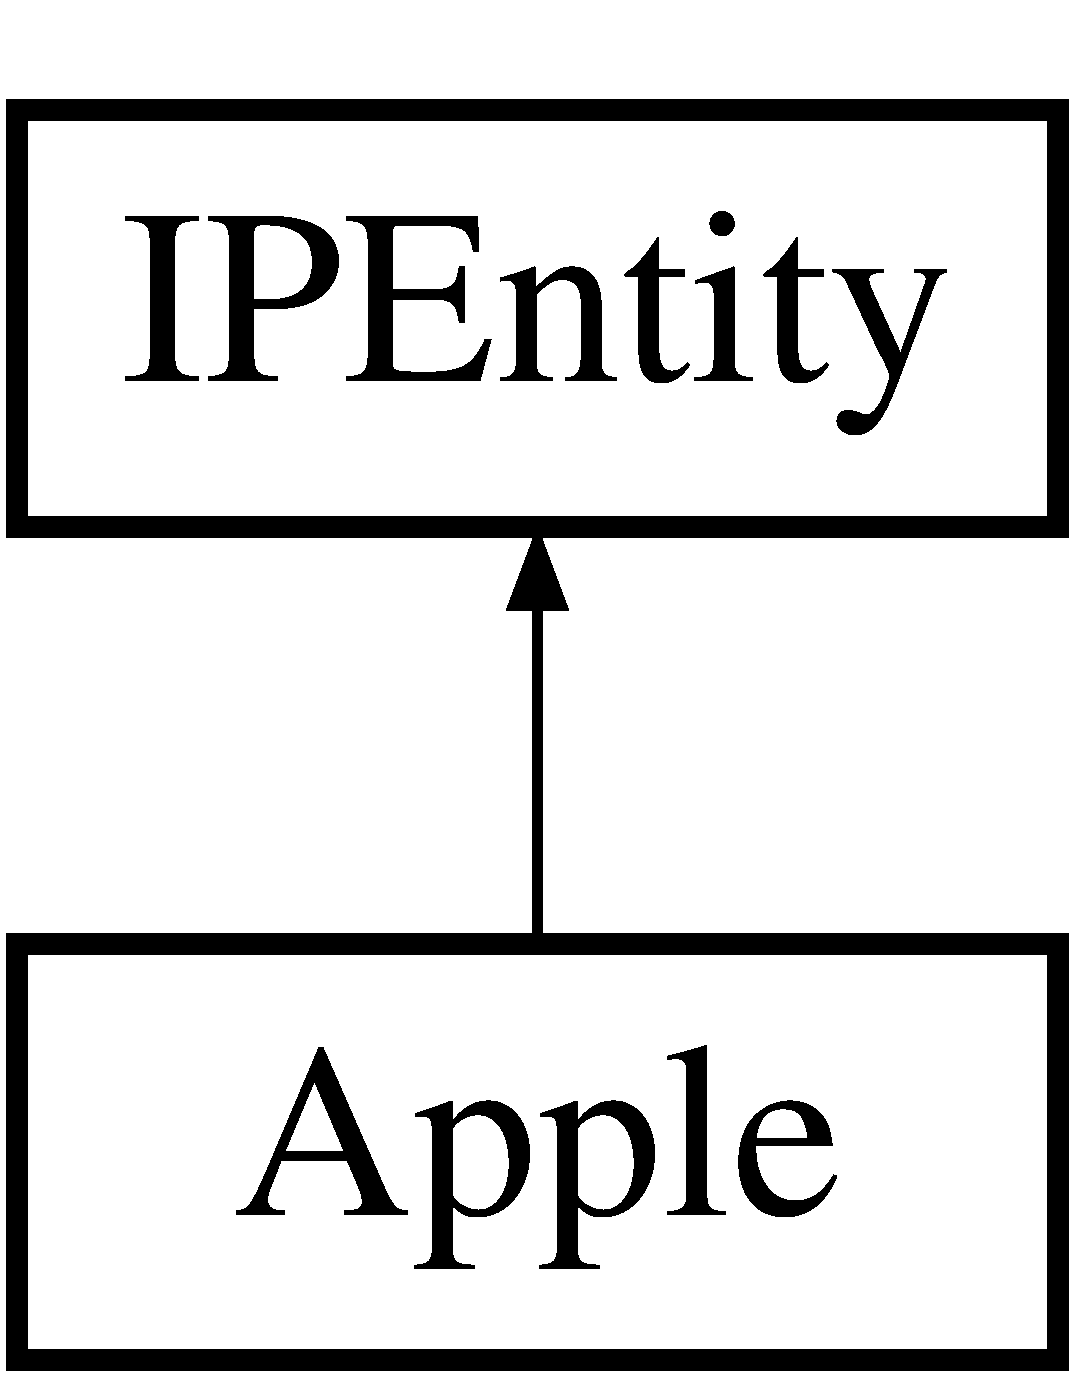
\includegraphics[height=2.000000cm]{class_apple}
\end{center}
\end{figure}
\subsection*{Public Member Functions}
\begin{DoxyCompactItemize}
\item 
\mbox{\Hypertarget{class_apple_af4e679170655408240a317e099f3e1d6}\label{class_apple_af4e679170655408240a317e099f3e1d6}} 
{\bfseries Apple} (\hyperlink{struct_vector2}{Vector2}$<$ int $>$ pos)
\item 
\mbox{\Hypertarget{class_apple_ad996f13370cbc05c25b60aa870f2aa66}\label{class_apple_ad996f13370cbc05c25b60aa870f2aa66}} 
\hyperlink{struct_vector2}{Vector2}$<$ int $>$ {\bfseries get\+Position} ()
\item 
\mbox{\Hypertarget{class_apple_a394bd2a13137cb232187d1952e100418}\label{class_apple_a394bd2a13137cb232187d1952e100418}} 
std\+::string {\bfseries get\+Name} ()
\item 
\mbox{\Hypertarget{class_apple_a5a31a10338aa5da199b4bfa91094b15a}\label{class_apple_a5a31a10338aa5da199b4bfa91094b15a}} 
std\+::string {\bfseries get\+Color} ()
\end{DoxyCompactItemize}


The documentation for this class was generated from the following files\+:\begin{DoxyCompactItemize}
\item 
games/\+Pac\+Man/Apple.\+hpp\item 
games/\+Pac\+Man/Apple.\+cpp\end{DoxyCompactItemize}

\hypertarget{class_arcade_exception}{}\section{Arcade\+Exception Class Reference}
\label{class_arcade_exception}\index{Arcade\+Exception@{Arcade\+Exception}}
Inheritance diagram for Arcade\+Exception\+:\begin{figure}[H]
\begin{center}
\leavevmode
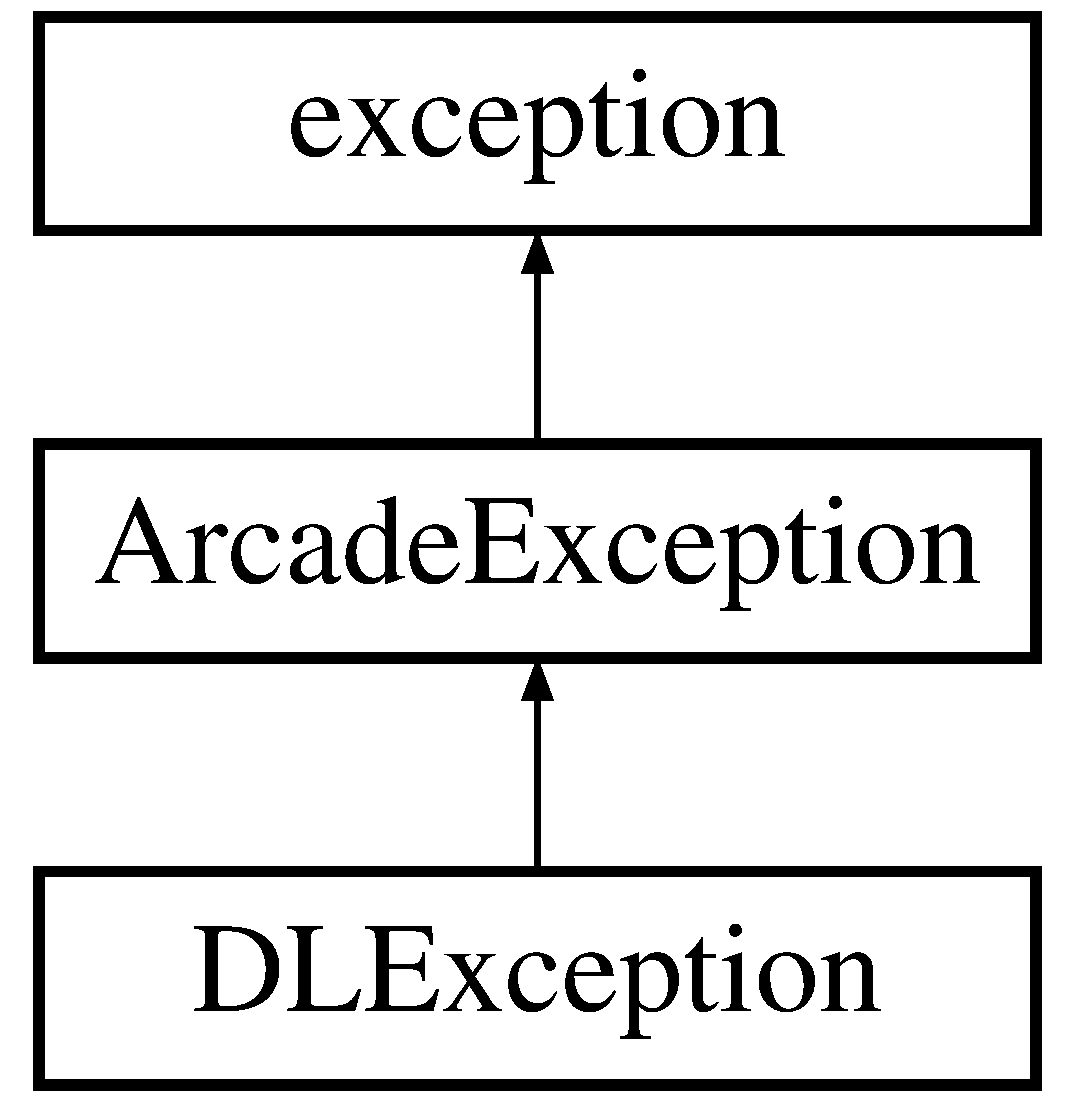
\includegraphics[height=3.000000cm]{class_arcade_exception}
\end{center}
\end{figure}
\subsection*{Public Member Functions}
\begin{DoxyCompactItemize}
\item 
\hyperlink{class_arcade_exception_ad7e357368a060f8becc46f68db639951}{Arcade\+Exception} (const std\+::string \&component, const std\+::string \&what)
\begin{DoxyCompactList}\small\item\em \hyperlink{class_arcade_exception}{Arcade\+Exception} Constructor. \end{DoxyCompactList}\item 
\mbox{\Hypertarget{class_arcade_exception_abbe1e647d775c7f8e3a4daba217b3514}\label{class_arcade_exception_abbe1e647d775c7f8e3a4daba217b3514}} 
const std\+::string \& {\bfseries Get\+Component} () const
\item 
\mbox{\Hypertarget{class_arcade_exception_ae8045bc16a31a859c210afea74de0797}\label{class_arcade_exception_ae8045bc16a31a859c210afea74de0797}} 
const char $\ast$ {\bfseries what} () const  throw ()
\end{DoxyCompactItemize}
\subsection*{Protected Attributes}
\begin{DoxyCompactItemize}
\item 
\mbox{\Hypertarget{class_arcade_exception_a3a5f7687d6090d2bbf7bb3d0421dbfe8}\label{class_arcade_exception_a3a5f7687d6090d2bbf7bb3d0421dbfe8}} 
const std\+::string {\bfseries \+\_\+component}
\item 
\mbox{\Hypertarget{class_arcade_exception_a499d9d1437e902595e5146c10c98dc4e}\label{class_arcade_exception_a499d9d1437e902595e5146c10c98dc4e}} 
const std\+::string {\bfseries \+\_\+what}
\end{DoxyCompactItemize}


\subsection{Constructor \& Destructor Documentation}
\mbox{\Hypertarget{class_arcade_exception_ad7e357368a060f8becc46f68db639951}\label{class_arcade_exception_ad7e357368a060f8becc46f68db639951}} 
\index{Arcade\+Exception@{Arcade\+Exception}!Arcade\+Exception@{Arcade\+Exception}}
\index{Arcade\+Exception@{Arcade\+Exception}!Arcade\+Exception@{Arcade\+Exception}}
\subsubsection{\texorpdfstring{Arcade\+Exception()}{ArcadeException()}}
{\footnotesize\ttfamily Arcade\+Exception\+::\+Arcade\+Exception (\begin{DoxyParamCaption}\item[{const std\+::string \&}]{component,  }\item[{const std\+::string \&}]{what }\end{DoxyParamCaption})}



\hyperlink{class_arcade_exception}{Arcade\+Exception} Constructor. 


\begin{DoxyParams}{Parameters}
{\em component} & Source of the exception \\
\hline
{\em what} & Error message for this exception\\
\hline
\end{DoxyParams}
\begin{DoxyReturn}{Returns}
New instance of \hyperlink{class_arcade_exception}{Arcade\+Exception} 
\end{DoxyReturn}


The documentation for this class was generated from the following files\+:\begin{DoxyCompactItemize}
\item 
core/\+Exceptions/Arcade\+Exception.\+hpp\item 
core/\+Exceptions/Arcade\+Exception.\+cpp\end{DoxyCompactItemize}

\hypertarget{class_camera}{}\section{Camera Class Reference}
\label{class_camera}\index{Camera@{Camera}}
\subsection*{Public Types}
\begin{DoxyCompactItemize}
\item 
\mbox{\Hypertarget{class_camera_a10b22bc796e45c0dd2518cce238f4878}\label{class_camera_a10b22bc796e45c0dd2518cce238f4878}} 
enum {\bfseries Cam\+Enum} \{ \newline
{\bfseries F\+R\+O\+NT}, 
{\bfseries B\+A\+CK}, 
{\bfseries R\+I\+G\+HT}, 
{\bfseries L\+E\+FT}, 
\newline
{\bfseries UP}, 
{\bfseries D\+O\+WN}, 
{\bfseries R\+O\+T\+\_\+X}, 
{\bfseries R\+O\+T\+\_\+Y}
 \}
\end{DoxyCompactItemize}
\subsection*{Public Member Functions}
\begin{DoxyCompactItemize}
\item 
\mbox{\Hypertarget{class_camera_a93e120c95f48fcc3a317b4dd318368b5}\label{class_camera_a93e120c95f48fcc3a317b4dd318368b5}} 
{\bfseries Camera} (const glm\+::vec3 \&position=glm\+::vec3(0.\+0f, 0.\+0f, 0.\+0f), const glm\+::vec3 \&rotation=glm\+::vec3(0.\+0f, 0.\+0f, 0.\+0f))
\item 
\mbox{\Hypertarget{class_camera_abf048471bef22e204b5d897c46503abf}\label{class_camera_abf048471bef22e204b5d897c46503abf}} 
void {\bfseries update\+View} (void)
\item 
\mbox{\Hypertarget{class_camera_a9a041ae11fa64b5edd843e0a98f8bebc}\label{class_camera_a9a041ae11fa64b5edd843e0a98f8bebc}} 
const glm\+::mat4 \& {\bfseries get\+View\+Matrix} (void) const
\item 
\mbox{\Hypertarget{class_camera_a07cf0b0b59c54d768e288f9b8290db51}\label{class_camera_a07cf0b0b59c54d768e288f9b8290db51}} 
const glm\+::vec3 \& {\bfseries get\+Front} (void) const
\item 
\mbox{\Hypertarget{class_camera_ace0d7f4531021d311c9adba9d085915c}\label{class_camera_ace0d7f4531021d311c9adba9d085915c}} 
const glm\+::vec3 \& {\bfseries get\+Top} (void) const
\item 
\mbox{\Hypertarget{class_camera_a9f3ce98d151484af91ae5281e517753e}\label{class_camera_a9f3ce98d151484af91ae5281e517753e}} 
const float {\bfseries get\+Delta\+Time} (void)
\item 
\mbox{\Hypertarget{class_camera_a6c80882e87be75bde67f432ca3b21607}\label{class_camera_a6c80882e87be75bde67f432ca3b21607}} 
void {\bfseries set\+Position} (const glm\+::vec3 \&position)
\item 
\mbox{\Hypertarget{class_camera_afb765b3e938107102cc855ff5dde2248}\label{class_camera_afb765b3e938107102cc855ff5dde2248}} 
void {\bfseries set\+Rotation} (const glm\+::vec3 \&rotation)
\item 
\mbox{\Hypertarget{class_camera_a4e1d6d8c4640a37cbdc93cf03c8ead42}\label{class_camera_a4e1d6d8c4640a37cbdc93cf03c8ead42}} 
void {\bfseries translate\+Camera} (const glm\+::vec3 \&translation)
\item 
\mbox{\Hypertarget{class_camera_ac37e0a9bc966151c94607a4ef57f750a}\label{class_camera_ac37e0a9bc966151c94607a4ef57f750a}} 
void {\bfseries rotate\+Camera} (const glm\+::vec3 \&rotation)
\item 
\mbox{\Hypertarget{class_camera_a5a3b649297187b0cb38256dd193df84e}\label{class_camera_a5a3b649297187b0cb38256dd193df84e}} 
void {\bfseries move} (const Cam\+Enum \&direction, const float \&speed)
\item 
\mbox{\Hypertarget{class_camera_a1fcaf262ca8a781b8a43ae8243ef7a12}\label{class_camera_a1fcaf262ca8a781b8a43ae8243ef7a12}} 
void {\bfseries rotate} (const Cam\+Enum \&axis, const float \&angle)
\end{DoxyCompactItemize}


The documentation for this class was generated from the following files\+:\begin{DoxyCompactItemize}
\item 
lib/\+Open\+G\+L/classes/Camera.\+hpp\item 
lib/\+Open\+G\+L/classes/Camera.\+cpp\end{DoxyCompactItemize}

\hypertarget{class_coin}{}\section{Coin Class Reference}
\label{class_coin}\index{Coin@{Coin}}
Inheritance diagram for Coin\+:\begin{figure}[H]
\begin{center}
\leavevmode
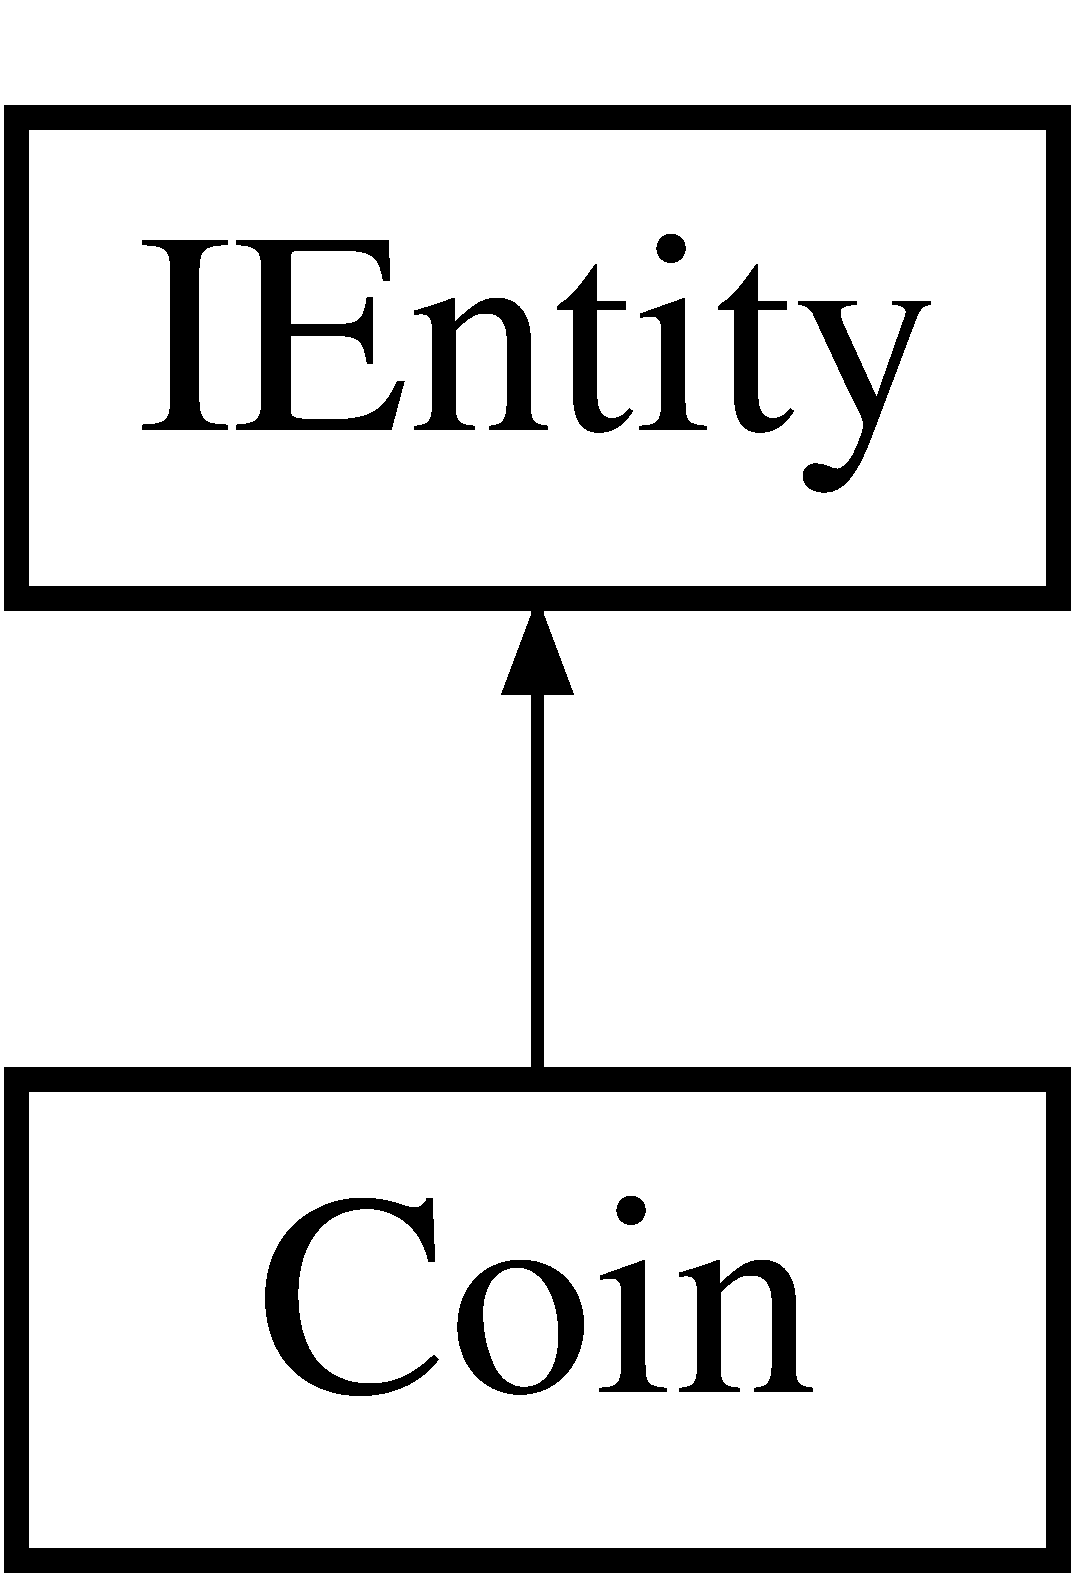
\includegraphics[height=2.000000cm]{class_coin}
\end{center}
\end{figure}
\subsection*{Public Member Functions}
\begin{DoxyCompactItemize}
\item 
\mbox{\Hypertarget{class_coin_a5cf3ac1d050f0a6719cda865a64bfd50}\label{class_coin_a5cf3ac1d050f0a6719cda865a64bfd50}} 
std\+::string {\bfseries get\+Name} () final
\item 
\mbox{\Hypertarget{class_coin_a337dd575cb8929d5f4f270edc18ac977}\label{class_coin_a337dd575cb8929d5f4f270edc18ac977}} 
std\+::string {\bfseries get\+Color} () final
\end{DoxyCompactItemize}


The documentation for this class was generated from the following files\+:\begin{DoxyCompactItemize}
\item 
games/\+Snake/Coin.\+hpp\item 
games/\+Snake/Coin.\+cpp\end{DoxyCompactItemize}

\hypertarget{struct_color}{}\section{Color Struct Reference}
\label{struct_color}\index{Color@{Color}}
\subsection*{Public Member Functions}
\begin{DoxyCompactItemize}
\item 
\mbox{\Hypertarget{struct_color_a72044de8fa4875bd7539515bdaa7eb9c}\label{struct_color_a72044de8fa4875bd7539515bdaa7eb9c}} 
{\bfseries Color} (const int \&\+\_\+r, const int \&\+\_\+g, const int \&\+\_\+b, const int \&\+\_\+a)
\item 
\mbox{\Hypertarget{struct_color_a54f0af3c549ccb609e1f217b9e192622}\label{struct_color_a54f0af3c549ccb609e1f217b9e192622}} 
{\bfseries Color} (const sf\+::\+Color \&color)
\end{DoxyCompactItemize}
\subsection*{Public Attributes}
\begin{DoxyCompactItemize}
\item 
\mbox{\Hypertarget{struct_color_a4954bdc9772da2a610401b8a438125cb}\label{struct_color_a4954bdc9772da2a610401b8a438125cb}} 
int {\bfseries r}
\item 
\mbox{\Hypertarget{struct_color_ae11f00d34bf3ecd8c8278f68876b82bf}\label{struct_color_ae11f00d34bf3ecd8c8278f68876b82bf}} 
int {\bfseries b}
\item 
\mbox{\Hypertarget{struct_color_ab5656e995bddd43d286c7ff5629a31dd}\label{struct_color_ab5656e995bddd43d286c7ff5629a31dd}} 
int {\bfseries g}
\item 
\mbox{\Hypertarget{struct_color_aa85f0a7c4980f26d7799dbbc8c1f7aa2}\label{struct_color_aa85f0a7c4980f26d7799dbbc8c1f7aa2}} 
int {\bfseries a}
\end{DoxyCompactItemize}


The documentation for this struct was generated from the following file\+:\begin{DoxyCompactItemize}
\item 
lib/\+Templates/Color.\+hpp\end{DoxyCompactItemize}

\hypertarget{class_cube}{}\section{Cube Class Reference}
\label{class_cube}\index{Cube@{Cube}}
Inheritance diagram for Cube\+:\begin{figure}[H]
\begin{center}
\leavevmode
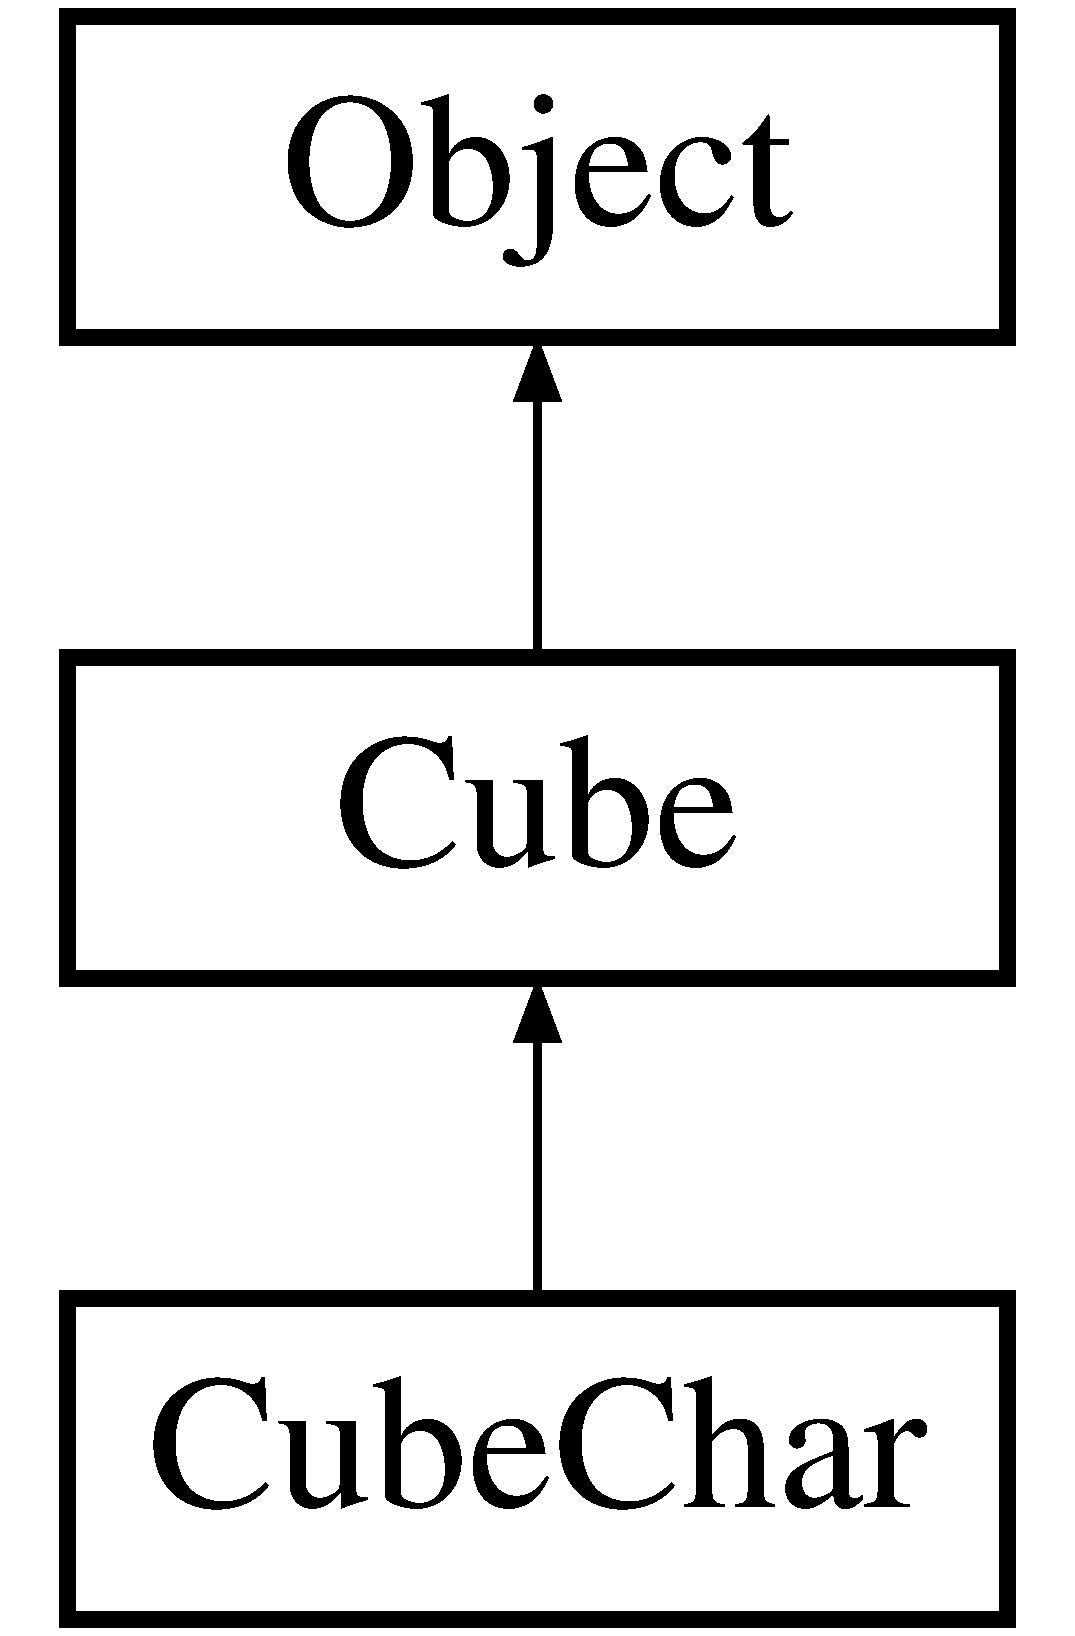
\includegraphics[height=3.000000cm]{class_cube}
\end{center}
\end{figure}
\subsection*{Public Member Functions}
\begin{DoxyCompactItemize}
\item 
\mbox{\Hypertarget{class_cube_a944189920558ba97a1a8a1e74f0403ec}\label{class_cube_a944189920558ba97a1a8a1e74f0403ec}} 
{\bfseries Cube} (const glm\+::vec3 \&position=glm\+::vec3(0.\+0f, 0.\+0f, 0.\+0f), const glm\+::vec3 \&rotation=glm\+::vec3(0.\+0f, 0.\+0f, 0.\+0f), const glm\+::vec3 \&scalation=glm\+::vec3(1.\+0f, 1.\+0f, 1.\+0f))
\end{DoxyCompactItemize}
\subsection*{Additional Inherited Members}


The documentation for this class was generated from the following files\+:\begin{DoxyCompactItemize}
\item 
lib/\+Open\+G\+L/classes/Cube.\+hpp\item 
lib/\+Open\+G\+L/classes/Cube.\+cpp\end{DoxyCompactItemize}

\hypertarget{class_cube_char}{}\section{Cube\+Char Class Reference}
\label{class_cube_char}\index{Cube\+Char@{Cube\+Char}}
Inheritance diagram for Cube\+Char\+:\begin{figure}[H]
\begin{center}
\leavevmode
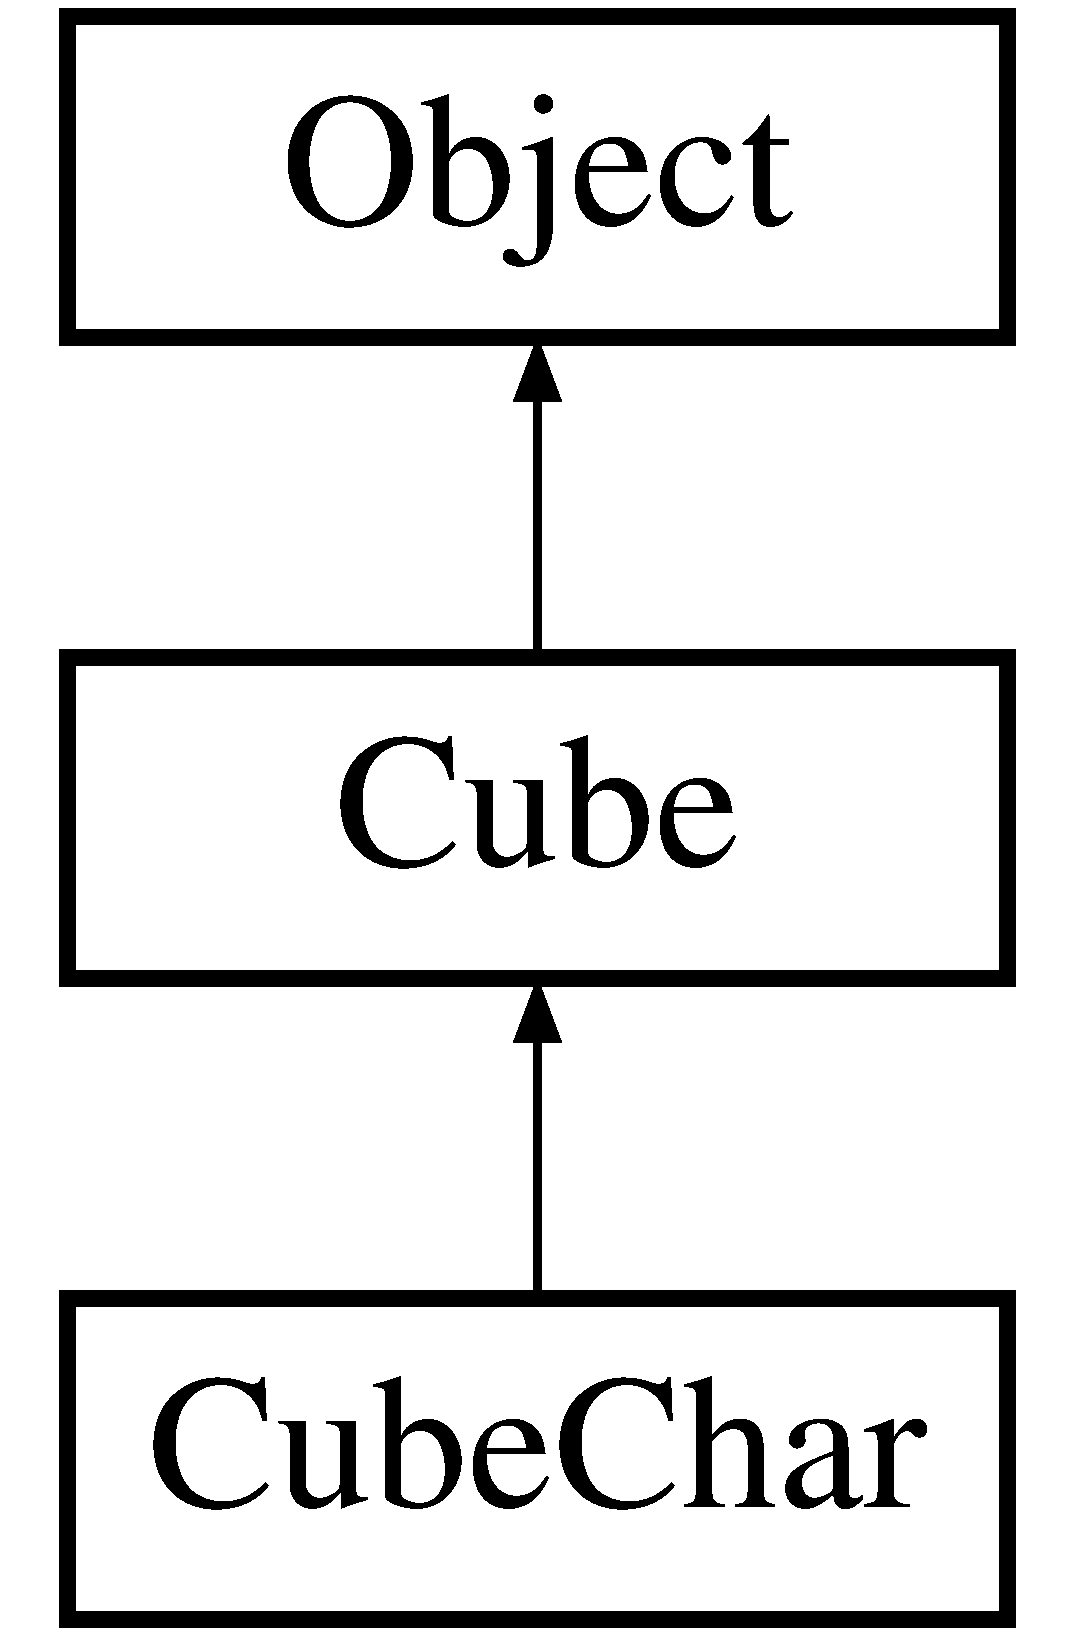
\includegraphics[height=3.000000cm]{class_cube_char}
\end{center}
\end{figure}
\subsection*{Public Member Functions}
\begin{DoxyCompactItemize}
\item 
\mbox{\Hypertarget{class_cube_char_af247c30c0f327f6324efd2218ea2cad3}\label{class_cube_char_af247c30c0f327f6324efd2218ea2cad3}} 
{\bfseries Cube\+Char} (const glm\+::vec3 \&position=glm\+::vec3(0.\+0f, 0.\+0f, 0.\+0f), const glm\+::vec3 \&rotation=glm\+::vec3(0.\+0f, 0.\+0f, 0.\+0f), const glm\+::vec3 \&scalation=glm\+::vec3(1.\+0f, 1.\+0f, 1.\+0f))
\item 
\mbox{\Hypertarget{class_cube_char_af72a46c8682f3f0c42c3e2feb1a7dcc7}\label{class_cube_char_af72a46c8682f3f0c42c3e2feb1a7dcc7}} 
void {\bfseries add\+Letter} (const char \&letter, const std\+::shared\+\_\+ptr$<$ \hyperlink{class_texture}{Texture} $>$ \&texture)
\item 
\mbox{\Hypertarget{class_cube_char_a6e527b86d64f804c9088d9f05b58e172}\label{class_cube_char_a6e527b86d64f804c9088d9f05b58e172}} 
const bool {\bfseries set\+Letter} (const char \&letter)
\end{DoxyCompactItemize}
\subsection*{Additional Inherited Members}


The documentation for this class was generated from the following files\+:\begin{DoxyCompactItemize}
\item 
lib/\+Open\+G\+L/classes/Cube\+Char.\+hpp\item 
lib/\+Open\+G\+L/classes/Cube\+Char.\+cpp\end{DoxyCompactItemize}

\hypertarget{class_d_l_exception}{}\section{D\+L\+Exception Class Reference}
\label{class_d_l_exception}\index{D\+L\+Exception@{D\+L\+Exception}}
Inheritance diagram for D\+L\+Exception\+:\begin{figure}[H]
\begin{center}
\leavevmode
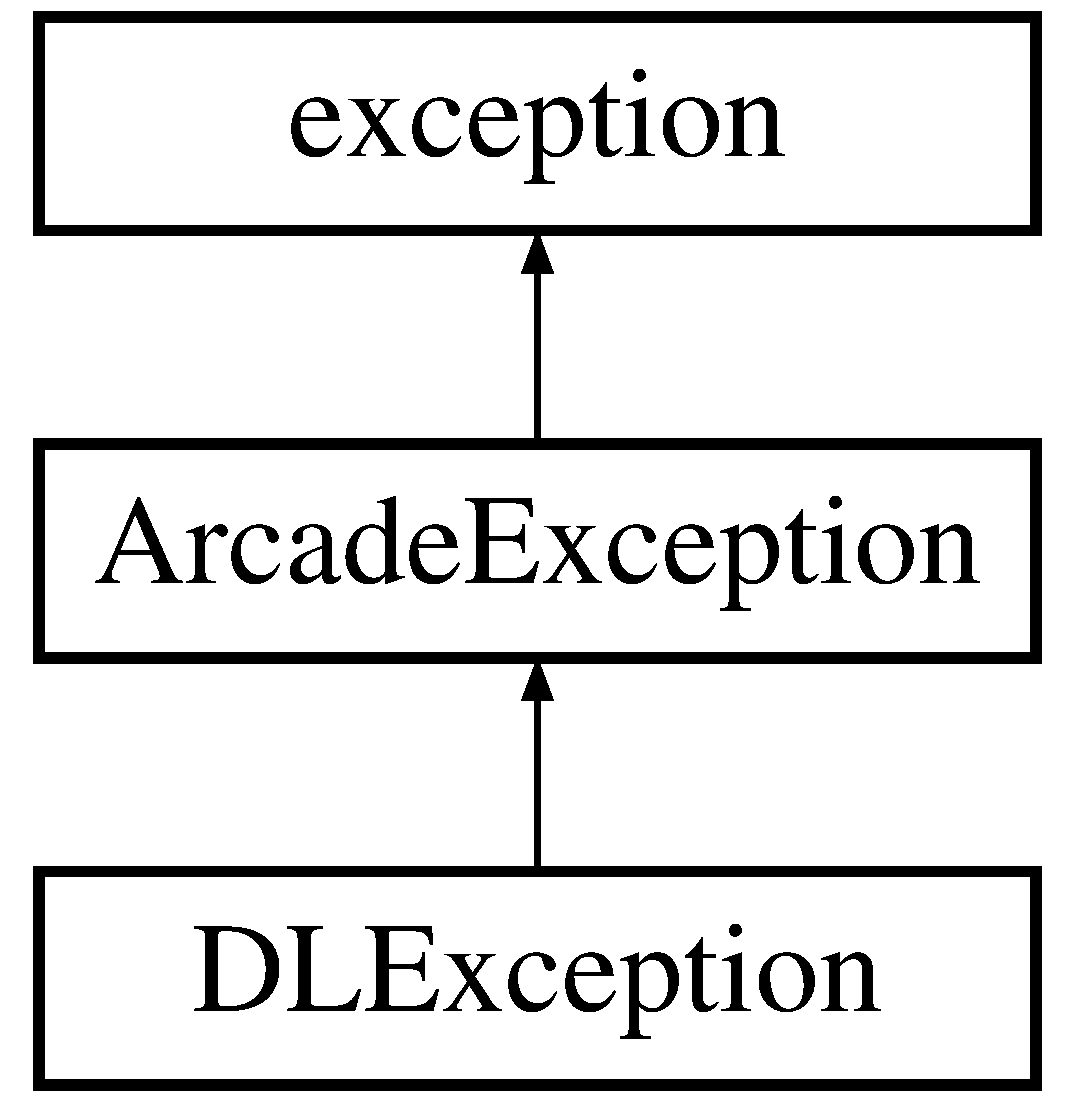
\includegraphics[height=3.000000cm]{class_d_l_exception}
\end{center}
\end{figure}
\subsection*{Public Member Functions}
\begin{DoxyCompactItemize}
\item 
\mbox{\Hypertarget{class_d_l_exception_ae1df8e8c9e64d1e3b2a9f36a758809a1}\label{class_d_l_exception_ae1df8e8c9e64d1e3b2a9f36a758809a1}} 
{\bfseries D\+L\+Exception} (const std\+::string \&component, const std\+::string \&what)
\end{DoxyCompactItemize}
\subsection*{Additional Inherited Members}


The documentation for this class was generated from the following files\+:\begin{DoxyCompactItemize}
\item 
core/\+Exceptions/Arcade\+Exception.\+hpp\item 
core/\+Exceptions/Arcade\+Exception.\+cpp\end{DoxyCompactItemize}

\hypertarget{class_d_l_loader}{}\section{D\+L\+Loader$<$ T $>$ Class Template Reference}
\label{class_d_l_loader}\index{D\+L\+Loader$<$ T $>$@{D\+L\+Loader$<$ T $>$}}
\subsection*{Public Member Functions}
\begin{DoxyCompactItemize}
\item 
\hyperlink{class_d_l_loader_ad4c7aee282549ba7064d3b539b9dca68}{D\+L\+Loader} (const std\+::string \&file, const Dynamic\+Library\+::\+Library\+Type \&type=Dynamic\+Library\+::\+Graphic)
\item 
T \& \hyperlink{class_d_l_loader_a7a023d81af75b962bddcef178b92e4c4}{Get\+Instance} ()
\begin{DoxyCompactList}\small\item\em Get instance of a Dynamic Library. \end{DoxyCompactList}\end{DoxyCompactItemize}


\subsection{Constructor \& Destructor Documentation}
\mbox{\Hypertarget{class_d_l_loader_ad4c7aee282549ba7064d3b539b9dca68}\label{class_d_l_loader_ad4c7aee282549ba7064d3b539b9dca68}} 
\index{D\+L\+Loader@{D\+L\+Loader}!D\+L\+Loader@{D\+L\+Loader}}
\index{D\+L\+Loader@{D\+L\+Loader}!D\+L\+Loader@{D\+L\+Loader}}
\subsubsection{\texorpdfstring{D\+L\+Loader()}{DLLoader()}}
{\footnotesize\ttfamily template$<$typename T $>$ \\
\hyperlink{class_d_l_loader}{D\+L\+Loader}$<$ T $>$\+::\hyperlink{class_d_l_loader}{D\+L\+Loader} (\begin{DoxyParamCaption}\item[{const std\+::string \&}]{file,  }\item[{const Dynamic\+Library\+::\+Library\+Type \&}]{type = {\ttfamily DynamicLibrary\+:\+:Graphic} }\end{DoxyParamCaption})}

Create and load an instance of a dynamic library


\begin{DoxyParams}{Parameters}
{\em file} & Path to dynamic library \\
\hline
{\em type} & Dynamic library type (Graphic or Game) \\
\hline
\end{DoxyParams}


\subsection{Member Function Documentation}
\mbox{\Hypertarget{class_d_l_loader_a7a023d81af75b962bddcef178b92e4c4}\label{class_d_l_loader_a7a023d81af75b962bddcef178b92e4c4}} 
\index{D\+L\+Loader@{D\+L\+Loader}!Get\+Instance@{Get\+Instance}}
\index{Get\+Instance@{Get\+Instance}!D\+L\+Loader@{D\+L\+Loader}}
\subsubsection{\texorpdfstring{Get\+Instance()}{GetInstance()}}
{\footnotesize\ttfamily template$<$typename T $>$ \\
T \& \hyperlink{class_d_l_loader}{D\+L\+Loader}$<$ T $>$\+::Get\+Instance (\begin{DoxyParamCaption}{ }\end{DoxyParamCaption})}



Get instance of a Dynamic Library. 

If the instance is null, an \hyperlink{class_arcade_exception}{Arcade\+Exception} is thrown.

\begin{DoxyReturn}{Returns}
A reference of type T to the instance of the Dynamic Library 
\end{DoxyReturn}


The documentation for this class was generated from the following files\+:\begin{DoxyCompactItemize}
\item 
core/\+D\+L\+Loader/D\+L\+Loader.\+hpp\item 
core/\+D\+L\+Loader/D\+L\+Loader.\+cpp\end{DoxyCompactItemize}

\hypertarget{class_dynamic_library}{}\section{Dynamic\+Library Class Reference}
\label{class_dynamic_library}\index{Dynamic\+Library@{Dynamic\+Library}}
\subsection*{Public Types}
\begin{DoxyCompactItemize}
\item 
\mbox{\Hypertarget{class_dynamic_library_afb8f6e78a2a72fb58501f4d1fb38ad3f}\label{class_dynamic_library_afb8f6e78a2a72fb58501f4d1fb38ad3f}} 
enum {\bfseries Library\+Type} \{ {\bfseries Graphic}, 
{\bfseries Game}
 \}
\end{DoxyCompactItemize}
\subsection*{Public Member Functions}
\begin{DoxyCompactItemize}
\item 
void $\ast$ \hyperlink{class_dynamic_library_afa5c94973f70976c400dd3caeafc6022}{Open} (const std\+::string \&file, const int \&flags)
\begin{DoxyCompactList}\small\item\em Open a Dynamic Library. \end{DoxyCompactList}\item 
const std\+::size\+\_\+t \hyperlink{class_dynamic_library_adb3b9207f5fcd9f00694af48a7e45cc9}{Close} (void $\ast$handle)
\begin{DoxyCompactList}\small\item\em Close a Dynamic Library using {\ttfamily dlclose()} \end{DoxyCompactList}\item 
void $\ast$ \hyperlink{class_dynamic_library_a7be5e4717bd16b25d6ddfde33941409c}{Get\+Symbol} (void $\ast$handle, const std\+::string \&symbol)
\begin{DoxyCompactList}\small\item\em Get a symbol from a Dynamic Library using {\ttfamily dlsym()} \end{DoxyCompactList}\end{DoxyCompactItemize}


\subsection{Member Function Documentation}
\mbox{\Hypertarget{class_dynamic_library_adb3b9207f5fcd9f00694af48a7e45cc9}\label{class_dynamic_library_adb3b9207f5fcd9f00694af48a7e45cc9}} 
\index{Dynamic\+Library@{Dynamic\+Library}!Close@{Close}}
\index{Close@{Close}!Dynamic\+Library@{Dynamic\+Library}}
\subsubsection{\texorpdfstring{Close()}{Close()}}
{\footnotesize\ttfamily const std\+::size\+\_\+t Dynamic\+Library\+::\+Close (\begin{DoxyParamCaption}\item[{void $\ast$}]{handle }\end{DoxyParamCaption})}



Close a Dynamic Library using {\ttfamily dlclose()} 

Close a Dynamic Library using {\ttfamily dlclose()} If {\ttfamily dlclose()} fail, a \hyperlink{class_d_l_exception}{D\+L\+Exception} is thrown. The error message contains {\ttfamily dlerror()} information


\begin{DoxyParams}{Parameters}
{\em handle} & A handle to a Dynamic Library\\
\hline
\end{DoxyParams}
\begin{DoxyReturn}{Returns}
-\/1 if handle is null, 0 otherwise 
\end{DoxyReturn}
\mbox{\Hypertarget{class_dynamic_library_a7be5e4717bd16b25d6ddfde33941409c}\label{class_dynamic_library_a7be5e4717bd16b25d6ddfde33941409c}} 
\index{Dynamic\+Library@{Dynamic\+Library}!Get\+Symbol@{Get\+Symbol}}
\index{Get\+Symbol@{Get\+Symbol}!Dynamic\+Library@{Dynamic\+Library}}
\subsubsection{\texorpdfstring{Get\+Symbol()}{GetSymbol()}}
{\footnotesize\ttfamily void $\ast$ Dynamic\+Library\+::\+Get\+Symbol (\begin{DoxyParamCaption}\item[{void $\ast$}]{handle,  }\item[{const std\+::string \&}]{symbol }\end{DoxyParamCaption})}



Get a symbol from a Dynamic Library using {\ttfamily dlsym()} 

Get a pointer to a function of the Dynamic Library


\begin{DoxyParams}{Parameters}
{\em handle} & A handle to a Dynamic Library \\
\hline
{\em symbol} & Function name\\
\hline
\end{DoxyParams}
\begin{DoxyReturn}{Returns}
A pointer to the function 
\end{DoxyReturn}
\mbox{\Hypertarget{class_dynamic_library_afa5c94973f70976c400dd3caeafc6022}\label{class_dynamic_library_afa5c94973f70976c400dd3caeafc6022}} 
\index{Dynamic\+Library@{Dynamic\+Library}!Open@{Open}}
\index{Open@{Open}!Dynamic\+Library@{Dynamic\+Library}}
\subsubsection{\texorpdfstring{Open()}{Open()}}
{\footnotesize\ttfamily void $\ast$ Dynamic\+Library\+::\+Open (\begin{DoxyParamCaption}\item[{const std\+::string \&}]{file,  }\item[{const int \&}]{flags }\end{DoxyParamCaption})}



Open a Dynamic Library. 

Open a Dynamic Library using {\ttfamily dlopen()} If {\ttfamily dlopen()} fail, a \hyperlink{class_d_l_exception}{D\+L\+Exception} is thrown. The error message contains {\ttfamily dlerror()} information


\begin{DoxyParams}{Parameters}
{\em file} & Path to .so file \\
\hline
{\em flags} & Flags to use with {\ttfamily dlopen()}\\
\hline
\end{DoxyParams}
\begin{DoxyReturn}{Returns}
A pointer to the beginning of the Dynamic Library 
\end{DoxyReturn}


The documentation for this class was generated from the following files\+:\begin{DoxyCompactItemize}
\item 
core/\+Dynamic\+Library/Dynamic\+Library.\+hpp\item 
core/\+Dynamic\+Library/Dynamic\+Library.\+cpp\end{DoxyCompactItemize}

\hypertarget{class_game_module}{}\section{Game\+Module Class Reference}
\label{class_game_module}\index{Game\+Module@{Game\+Module}}
Inheritance diagram for Game\+Module\+:\begin{figure}[H]
\begin{center}
\leavevmode
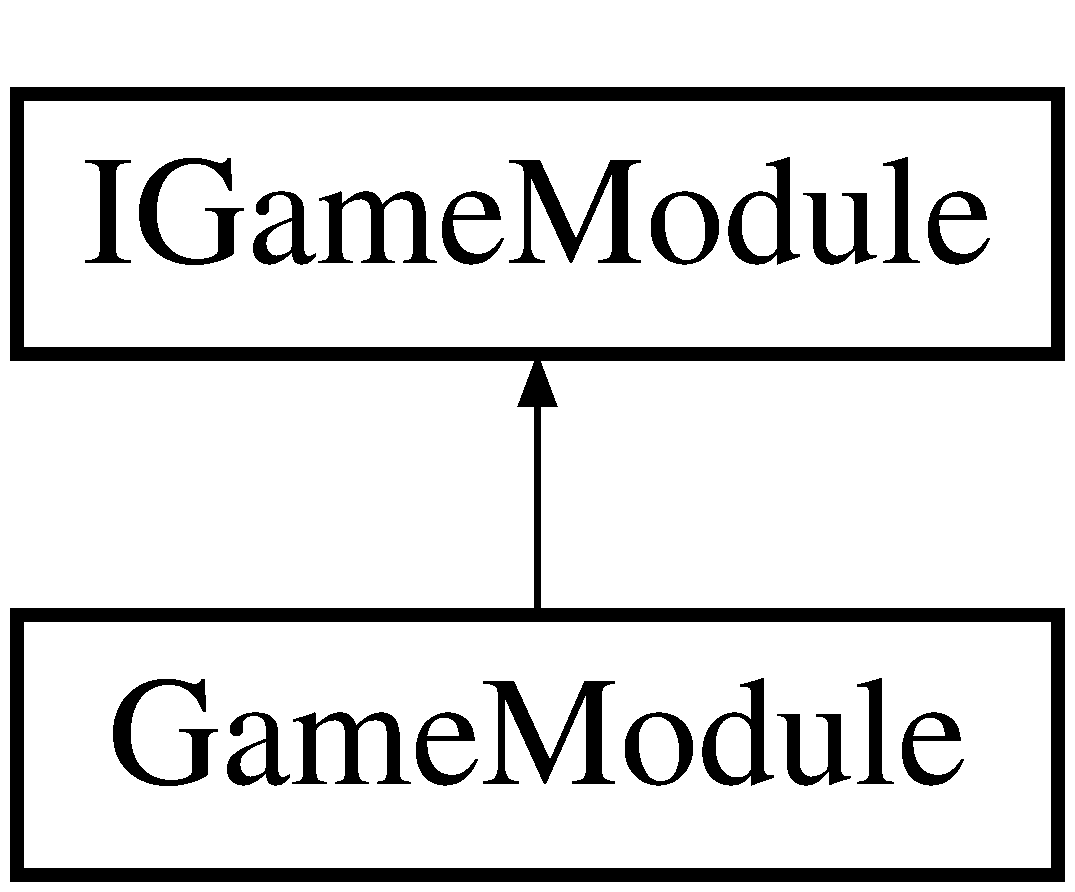
\includegraphics[height=2.000000cm]{class_game_module}
\end{center}
\end{figure}
\subsection*{Public Member Functions}
\begin{DoxyCompactItemize}
\item 
\hyperlink{class_game_module_a9d2cc872e80e4107d7f87818e9ea5455}{Game\+Module} (const std\+::string \&path)
\begin{DoxyCompactList}\small\item\em \hyperlink{class_game_module}{Game\+Module} constructor. \end{DoxyCompactList}\item 
const std\+::vector$<$ std\+::string $>$ \hyperlink{class_game_module_ab82644e3a4e4a5aa41c4f8e9c6077af7}{get\+Instruction} (std\+::string input) const
\begin{DoxyCompactList}\small\item\em Get instructions to execute from the game. \end{DoxyCompactList}\item 
const std\+::vector$<$ std\+::string $>$ \hyperlink{class_game_module_a54c7d41e2ddf42b1c46846f2653ad746}{get\+Textures} (void) const
\begin{DoxyCompactList}\small\item\em Get textures from the game. \end{DoxyCompactList}\item 
\mbox{\Hypertarget{class_game_module_a475400a8ee4a8183e3639c6cbeda47b1}\label{class_game_module_a475400a8ee4a8183e3639c6cbeda47b1}} 
const std\+::string {\bfseries get\+Name} (void)
\end{DoxyCompactItemize}


\subsection{Constructor \& Destructor Documentation}
\mbox{\Hypertarget{class_game_module_a9d2cc872e80e4107d7f87818e9ea5455}\label{class_game_module_a9d2cc872e80e4107d7f87818e9ea5455}} 
\index{Game\+Module@{Game\+Module}!Game\+Module@{Game\+Module}}
\index{Game\+Module@{Game\+Module}!Game\+Module@{Game\+Module}}
\subsubsection{\texorpdfstring{Game\+Module()}{GameModule()}}
{\footnotesize\ttfamily Game\+Module\+::\+Game\+Module (\begin{DoxyParamCaption}\item[{const std\+::string \&}]{path }\end{DoxyParamCaption})}



\hyperlink{class_game_module}{Game\+Module} constructor. 

Load the game passed as parameter using \hyperlink{class_d_l_loader}{D\+L\+Loader}


\begin{DoxyParams}{Parameters}
{\em path} & Path to the game library .so\\
\hline
\end{DoxyParams}
\begin{DoxyReturn}{Returns}
New instance of \hyperlink{class_game_module}{Game\+Module} 
\end{DoxyReturn}


\subsection{Member Function Documentation}
\mbox{\Hypertarget{class_game_module_ab82644e3a4e4a5aa41c4f8e9c6077af7}\label{class_game_module_ab82644e3a4e4a5aa41c4f8e9c6077af7}} 
\index{Game\+Module@{Game\+Module}!get\+Instruction@{get\+Instruction}}
\index{get\+Instruction@{get\+Instruction}!Game\+Module@{Game\+Module}}
\subsubsection{\texorpdfstring{get\+Instruction()}{getInstruction()}}
{\footnotesize\ttfamily const std\+::vector$<$ std\+::string $>$ Game\+Module\+::get\+Instruction (\begin{DoxyParamCaption}\item[{std\+::string}]{input }\end{DoxyParamCaption}) const}



Get instructions to execute from the game. 


\begin{DoxyParams}{Parameters}
{\em input} & User input \\
\hline
\end{DoxyParams}
\begin{DoxyReturn}{Returns}
A std\+::vector$<$std\+::string$>$ containing instructions 
\end{DoxyReturn}
\mbox{\Hypertarget{class_game_module_a54c7d41e2ddf42b1c46846f2653ad746}\label{class_game_module_a54c7d41e2ddf42b1c46846f2653ad746}} 
\index{Game\+Module@{Game\+Module}!get\+Textures@{get\+Textures}}
\index{get\+Textures@{get\+Textures}!Game\+Module@{Game\+Module}}
\subsubsection{\texorpdfstring{get\+Textures()}{getTextures()}}
{\footnotesize\ttfamily const std\+::vector$<$ std\+::string $>$ Game\+Module\+::get\+Textures (\begin{DoxyParamCaption}\item[{void}]{ }\end{DoxyParamCaption}) const}



Get textures from the game. 

Get all textures used in the game

\begin{DoxyReturn}{Returns}
A std\+::vector$<$std\+::string$>$ containing all textures 
\end{DoxyReturn}


The documentation for this class was generated from the following files\+:\begin{DoxyCompactItemize}
\item 
core/\+Game\+Module/Game\+Module.\+hpp\item 
core/\+Game\+Module/Game\+Module.\+cpp\end{DoxyCompactItemize}

\hypertarget{class_ghost}{}\section{Ghost Class Reference}
\label{class_ghost}\index{Ghost@{Ghost}}
Inheritance diagram for Ghost\+:\begin{figure}[H]
\begin{center}
\leavevmode
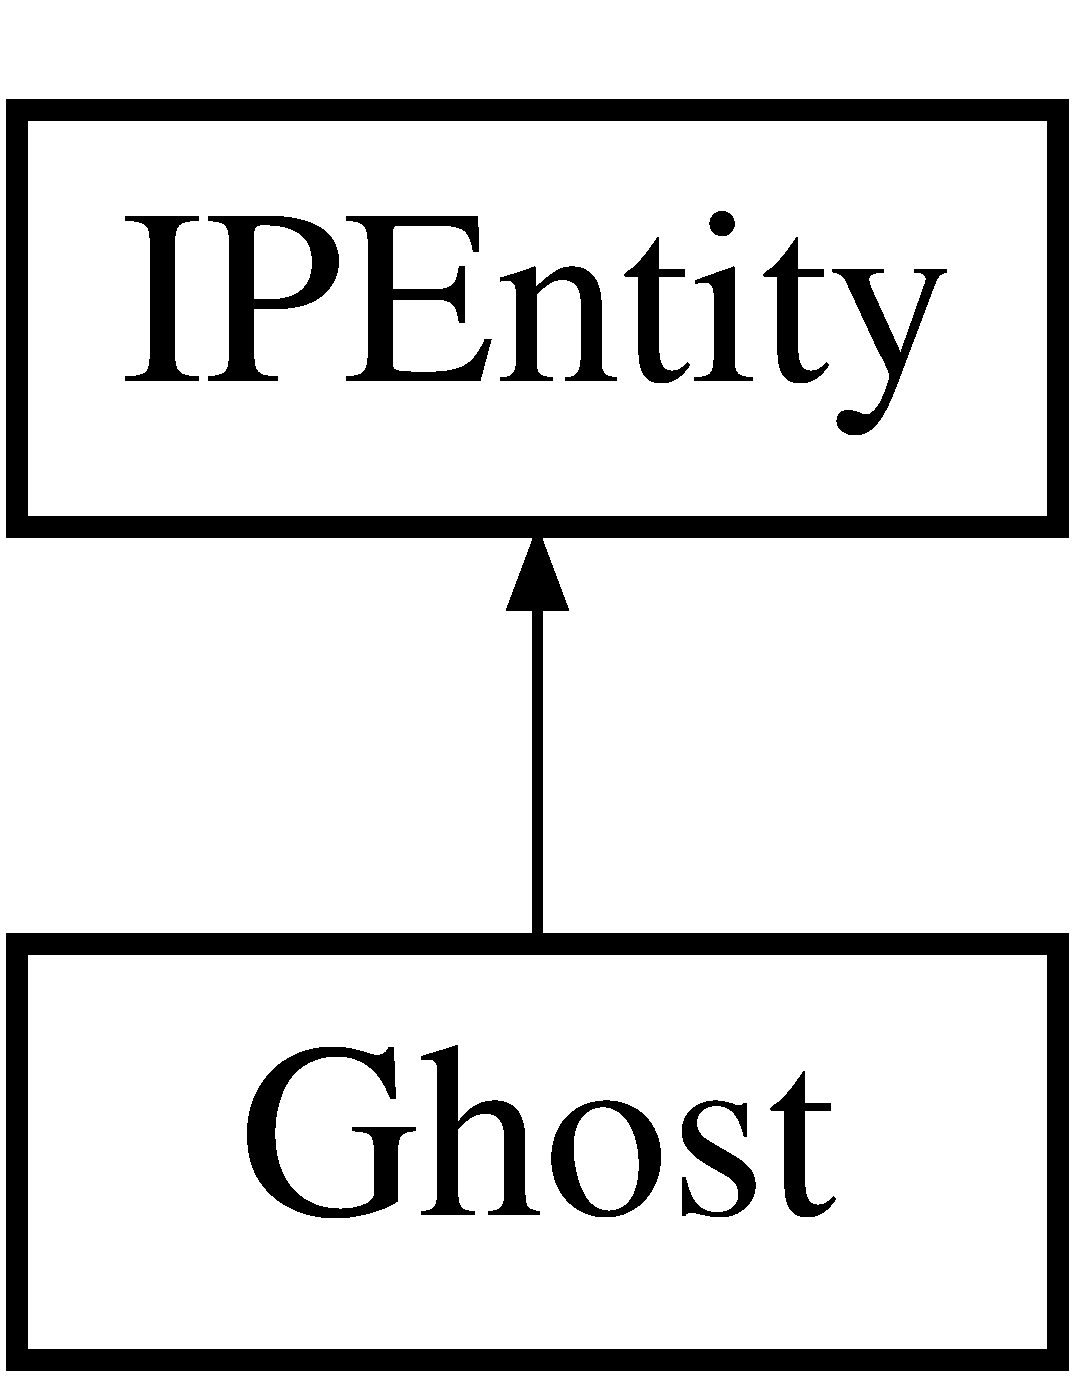
\includegraphics[height=2.000000cm]{class_ghost}
\end{center}
\end{figure}
\subsection*{Public Member Functions}
\begin{DoxyCompactItemize}
\item 
\mbox{\Hypertarget{class_ghost_ae0d5d21555c85c83dbbba12216a733ac}\label{class_ghost_ae0d5d21555c85c83dbbba12216a733ac}} 
{\bfseries Ghost} (\hyperlink{struct_vector2}{Vector2}$<$ int $>$ pos, \hyperlink{struct_vector2}{Vector2}$<$ int $>$ dir)
\item 
\mbox{\Hypertarget{class_ghost_a193bc3ec17d7d6592349d93dfc3616ca}\label{class_ghost_a193bc3ec17d7d6592349d93dfc3616ca}} 
\hyperlink{struct_vector2}{Vector2}$<$ int $>$ {\bfseries get\+Position} ()
\item 
\mbox{\Hypertarget{class_ghost_a7ce810b935588136b7240c35a1f039a1}\label{class_ghost_a7ce810b935588136b7240c35a1f039a1}} 
\hyperlink{struct_vector2}{Vector2}$<$ int $>$ {\bfseries get\+Dir} ()
\item 
\mbox{\Hypertarget{class_ghost_a4f91b2b32aab6edbbb4c76d2e0350526}\label{class_ghost_a4f91b2b32aab6edbbb4c76d2e0350526}} 
void {\bfseries set\+Dir} (\hyperlink{struct_vector2}{Vector2}$<$ int $>$ dir)
\item 
\mbox{\Hypertarget{class_ghost_af184febbc50b03c4ca265aee4820cddc}\label{class_ghost_af184febbc50b03c4ca265aee4820cddc}} 
void {\bfseries set\+Pos} (\hyperlink{struct_vector2}{Vector2}$<$ int $>$ dir)
\item 
\mbox{\Hypertarget{class_ghost_a6de989813477a1db9eac0fbe86327e36}\label{class_ghost_a6de989813477a1db9eac0fbe86327e36}} 
std\+::string {\bfseries get\+Name} ()
\item 
\mbox{\Hypertarget{class_ghost_a13cb35b14f25734e6ca388d96498bd95}\label{class_ghost_a13cb35b14f25734e6ca388d96498bd95}} 
std\+::string {\bfseries get\+Color} ()
\item 
\mbox{\Hypertarget{class_ghost_aeaed1e48a841710da0a01ca01e7a5fda}\label{class_ghost_aeaed1e48a841710da0a01ca01e7a5fda}} 
void {\bfseries set\+Uber} (bool)
\item 
\mbox{\Hypertarget{class_ghost_a231a741f4efcc40f47bddb7efa61a19d}\label{class_ghost_a231a741f4efcc40f47bddb7efa61a19d}} 
void {\bfseries move} ()
\item 
\mbox{\Hypertarget{class_ghost_a37f8ffa1a514de1cee88c16d8c2d56ed}\label{class_ghost_a37f8ffa1a514de1cee88c16d8c2d56ed}} 
bool {\bfseries get\+State} ()
\end{DoxyCompactItemize}


The documentation for this class was generated from the following files\+:\begin{DoxyCompactItemize}
\item 
games/\+Pac\+Man/Ghost.\+hpp\item 
games/\+Pac\+Man/Ghost.\+cpp\end{DoxyCompactItemize}

\hypertarget{class_g_l_manager}{}\section{G\+L\+Manager Class Reference}
\label{class_g_l_manager}\index{G\+L\+Manager@{G\+L\+Manager}}
\subsection*{Public Member Functions}
\begin{DoxyCompactItemize}
\item 
\mbox{\Hypertarget{class_g_l_manager_ad87bda8387bc538bc0c4340501040483}\label{class_g_l_manager_ad87bda8387bc538bc0c4340501040483}} 
S\+D\+L\+\_\+\+Window $\ast$ {\bfseries get\+Window} (void) const
\item 
\mbox{\Hypertarget{class_g_l_manager_abbf99309cf92c7824637604c449f60ca}\label{class_g_l_manager_abbf99309cf92c7824637604c449f60ca}} 
const glm\+::mat4 \& {\bfseries get\+Perspective\+Matrix} (void) const
\item 
\mbox{\Hypertarget{class_g_l_manager_abd3642ffde790a4bd20c182144ac3ef4}\label{class_g_l_manager_abd3642ffde790a4bd20c182144ac3ef4}} 
void {\bfseries init\+Window} (const std\+::string \&name, const int \&wid=800, const int \&len=600)
\item 
\mbox{\Hypertarget{class_g_l_manager_a5d7b1d2c08f4f16d75f968b629f1d3b5}\label{class_g_l_manager_a5d7b1d2c08f4f16d75f968b629f1d3b5}} 
void {\bfseries set\+Perpective\+Matrix} (const float \&angle, const float \&ratio, const float \&near\+Plane, const float \&far\+Plane)
\item 
\mbox{\Hypertarget{class_g_l_manager_a1a3fd00de3c709ab4b81b1a734f971f2}\label{class_g_l_manager_a1a3fd00de3c709ab4b81b1a734f971f2}} 
void {\bfseries clear\+Window} (const G\+Lclampf \&r=0.\+0f, const G\+Lclampf \&g=0.\+0f, const G\+Lclampf \&b=0.\+0f, const G\+Lclampf \&a=1.\+0f)
\item 
\mbox{\Hypertarget{class_g_l_manager_a290e1f4ce2656c82f9eadaf800c4598b}\label{class_g_l_manager_a290e1f4ce2656c82f9eadaf800c4598b}} 
const std\+::string {\bfseries handle\+Events} (const std\+::map$<$ S\+D\+L\+\_\+\+Keycode, std\+::string $>$ \&keymap, \hyperlink{class_camera}{Camera} \&cam)
\item 
\mbox{\Hypertarget{class_g_l_manager_af495168157244aa4f79a5cb96625b077}\label{class_g_l_manager_af495168157244aa4f79a5cb96625b077}} 
const bool {\bfseries handle\+Key\+Down} (const S\+D\+L\+\_\+\+Keysym \&key, \hyperlink{class_camera}{Camera} \&cam)
\item 
\mbox{\Hypertarget{class_g_l_manager_a57d63191667702ad02e057f48f10147d}\label{class_g_l_manager_a57d63191667702ad02e057f48f10147d}} 
void {\bfseries handle\+Key\+Up} (const S\+D\+L\+\_\+\+Keysym \&key, \hyperlink{class_camera}{Camera} \&cam)
\item 
\mbox{\Hypertarget{class_g_l_manager_a342c998f2325bbdd693c817e76b3dced}\label{class_g_l_manager_a342c998f2325bbdd693c817e76b3dced}} 
const std\+::string {\bfseries get\+Input\+Char} (std\+::string \&to\+Fill)
\end{DoxyCompactItemize}


The documentation for this class was generated from the following files\+:\begin{DoxyCompactItemize}
\item 
lib/\+Open\+G\+L/classes/G\+L\+Manager.\+hpp\item 
lib/\+Open\+G\+L/classes/G\+L\+Manager.\+cpp\end{DoxyCompactItemize}

\hypertarget{class_i_entity}{}\section{I\+Entity Class Reference}
\label{class_i_entity}\index{I\+Entity@{I\+Entity}}
Inheritance diagram for I\+Entity\+:\begin{figure}[H]
\begin{center}
\leavevmode
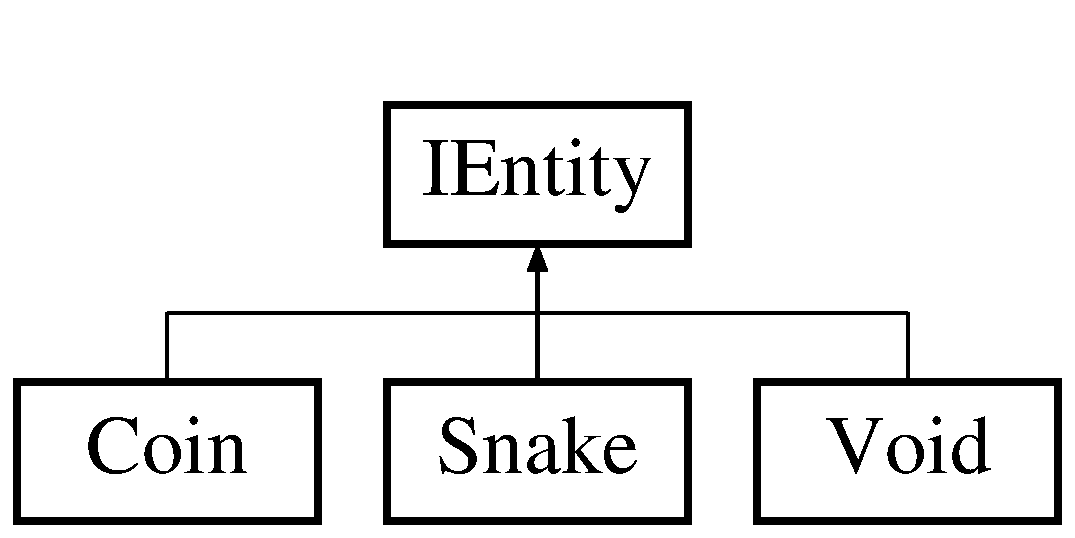
\includegraphics[height=2.000000cm]{class_i_entity}
\end{center}
\end{figure}
\subsection*{Public Member Functions}
\begin{DoxyCompactItemize}
\item 
\mbox{\Hypertarget{class_i_entity_adee9ecd717a48ac4cbbc11fb1e3c75cf}\label{class_i_entity_adee9ecd717a48ac4cbbc11fb1e3c75cf}} 
virtual std\+::string {\bfseries get\+Name} ()=0
\item 
\mbox{\Hypertarget{class_i_entity_a08b5f22489e8b78f3558414d86a3ec37}\label{class_i_entity_a08b5f22489e8b78f3558414d86a3ec37}} 
virtual std\+::string {\bfseries get\+Color} ()=0
\end{DoxyCompactItemize}


The documentation for this class was generated from the following file\+:\begin{DoxyCompactItemize}
\item 
games/\+Snake/I\+Entity.\+hpp\end{DoxyCompactItemize}

\hypertarget{class_i_game}{}\section{I\+Game Class Reference}
\label{class_i_game}\index{I\+Game@{I\+Game}}
Inheritance diagram for I\+Game\+:\begin{figure}[H]
\begin{center}
\leavevmode
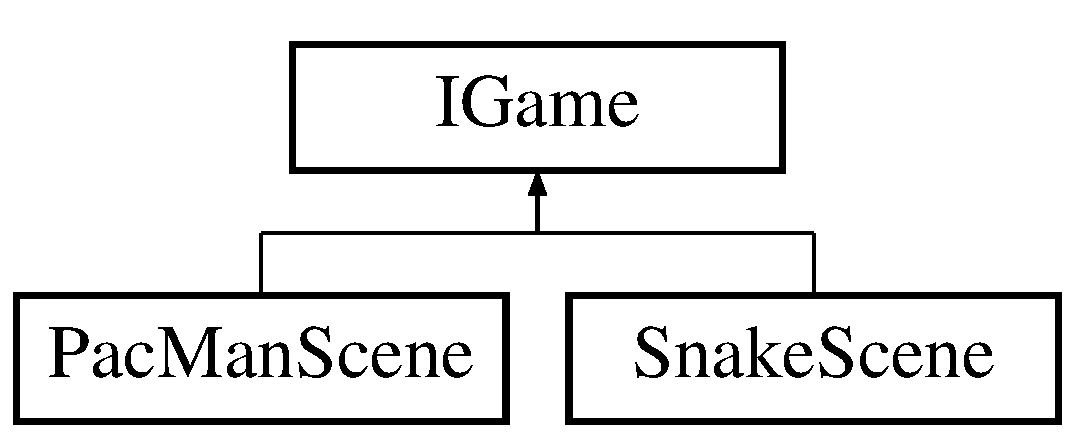
\includegraphics[height=2.000000cm]{class_i_game}
\end{center}
\end{figure}
\subsection*{Public Member Functions}
\begin{DoxyCompactItemize}
\item 
\mbox{\Hypertarget{class_i_game_a143a6acaa498c08964089c293fbaecba}\label{class_i_game_a143a6acaa498c08964089c293fbaecba}} 
virtual std\+::vector$<$ std\+::string $>$ {\bfseries Send\+Instruction} ()=0
\item 
\mbox{\Hypertarget{class_i_game_a46b64ca02a645790bbd83d9c7aa28cec}\label{class_i_game_a46b64ca02a645790bbd83d9c7aa28cec}} 
virtual std\+::vector$<$ std\+::string $>$ {\bfseries get\+Textures} ()=0
\item 
\mbox{\Hypertarget{class_i_game_aa3488c71c14dac53703e8debab91b503}\label{class_i_game_aa3488c71c14dac53703e8debab91b503}} 
virtual void {\bfseries update} (const std\+::string \&input)=0
\item 
\mbox{\Hypertarget{class_i_game_a43bfc6eee8384673e768016b7082c264}\label{class_i_game_a43bfc6eee8384673e768016b7082c264}} 
virtual std\+::string {\bfseries get\+Name} ()=0
\end{DoxyCompactItemize}


The documentation for this class was generated from the following file\+:\begin{DoxyCompactItemize}
\item 
games/I\+Game.\+hpp\end{DoxyCompactItemize}

\hypertarget{class_i_game_module}{}\section{I\+Game\+Module Class Reference}
\label{class_i_game_module}\index{I\+Game\+Module@{I\+Game\+Module}}
Inheritance diagram for I\+Game\+Module\+:\begin{figure}[H]
\begin{center}
\leavevmode
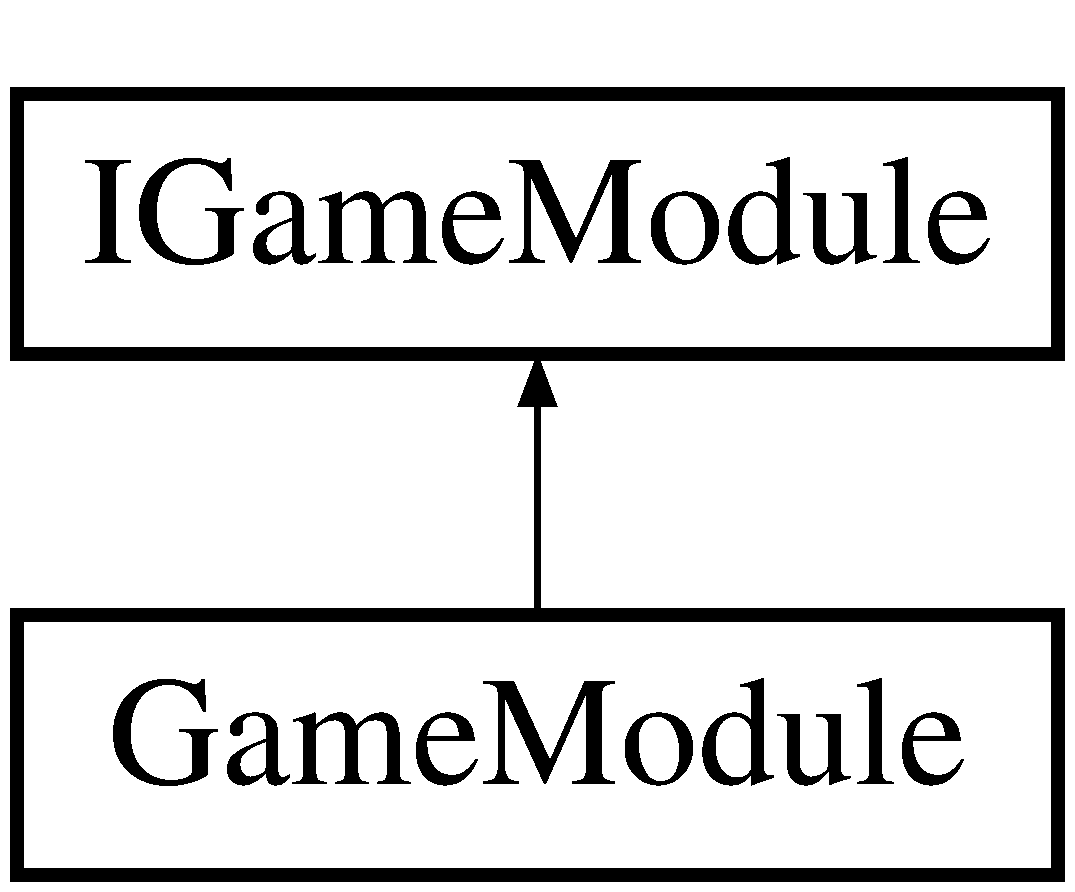
\includegraphics[height=2.000000cm]{class_i_game_module}
\end{center}
\end{figure}


The documentation for this class was generated from the following file\+:\begin{DoxyCompactItemize}
\item 
core/\+Game\+Module/I\+Game\+Module.\+hpp\end{DoxyCompactItemize}

\hypertarget{class_i_graphics}{}\section{I\+Graphics Class Reference}
\label{class_i_graphics}\index{I\+Graphics@{I\+Graphics}}
Inheritance diagram for I\+Graphics\+:\begin{figure}[H]
\begin{center}
\leavevmode
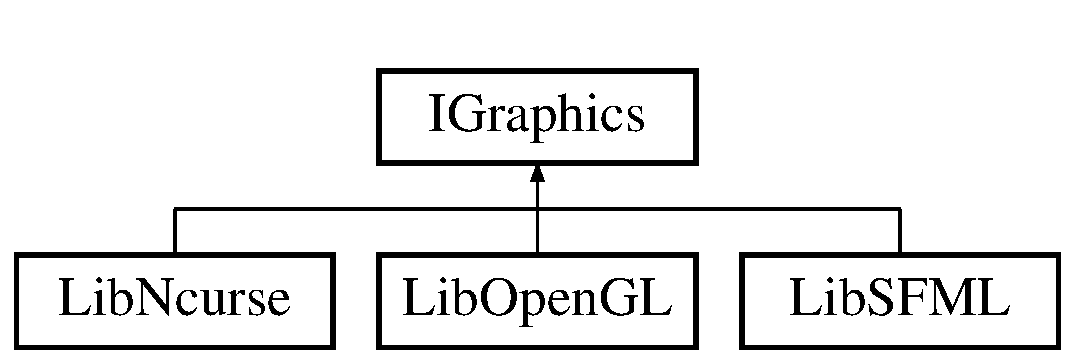
\includegraphics[height=2.000000cm]{class_i_graphics}
\end{center}
\end{figure}
\subsection*{Public Member Functions}
\begin{DoxyCompactItemize}
\item 
\mbox{\Hypertarget{class_i_graphics_a7d56d29cf685199d3369d9e2a35ee531}\label{class_i_graphics_a7d56d29cf685199d3369d9e2a35ee531}} 
virtual void {\bfseries Init} ()=0
\item 
\mbox{\Hypertarget{class_i_graphics_a13387f73d81f2e66127cc317febb6e8a}\label{class_i_graphics_a13387f73d81f2e66127cc317febb6e8a}} 
virtual void {\bfseries draw\+Rectangle} (const \hyperlink{struct_rectangle}{Rectangle}$<$ int $>$ \&rect, const std\+::string \&color)=0
\item 
\mbox{\Hypertarget{class_i_graphics_a2d49395b7140d1348f739535b5412eea}\label{class_i_graphics_a2d49395b7140d1348f739535b5412eea}} 
virtual void {\bfseries draw\+Window} (void)=0
\item 
\mbox{\Hypertarget{class_i_graphics_a1e3e1573e3fd226f5b939ed32083ba20}\label{class_i_graphics_a1e3e1573e3fd226f5b939ed32083ba20}} 
virtual const std\+::string {\bfseries handle\+Event} (void)=0
\item 
\mbox{\Hypertarget{class_i_graphics_a27551effcc2af1f9071a30a466ad09c8}\label{class_i_graphics_a27551effcc2af1f9071a30a466ad09c8}} 
virtual void {\bfseries draw\+Text} (const std\+::string \&text, const \hyperlink{struct_vector2}{Vector2}$<$ int $>$ \&position, const std\+::string \&color)=0
\item 
\mbox{\Hypertarget{class_i_graphics_a380e9d5db4f52905a73d3d0a12b880f0}\label{class_i_graphics_a380e9d5db4f52905a73d3d0a12b880f0}} 
virtual void {\bfseries clear\+Window} (void)=0
\item 
\mbox{\Hypertarget{class_i_graphics_a9d8f215aba1b8cda8d1a4b87e9cb3eaa}\label{class_i_graphics_a9d8f215aba1b8cda8d1a4b87e9cb3eaa}} 
virtual void {\bfseries enter\+Text\+Mode} ()=0
\item 
\mbox{\Hypertarget{class_i_graphics_a5c3bf577570c5447f6e8f2eeffc08933}\label{class_i_graphics_a5c3bf577570c5447f6e8f2eeffc08933}} 
virtual void {\bfseries load\+Textures} (std\+::vector$<$ std\+::string $>$)=0
\item 
\mbox{\Hypertarget{class_i_graphics_a0da7a8862b6cc41046edee979be9faa8}\label{class_i_graphics_a0da7a8862b6cc41046edee979be9faa8}} 
virtual void {\bfseries close} ()=0
\item 
\mbox{\Hypertarget{class_i_graphics_a785e4c5f06c8e1a21028581f8cd76f5d}\label{class_i_graphics_a785e4c5f06c8e1a21028581f8cd76f5d}} 
virtual const bool {\bfseries is\+Open} () const =0
\end{DoxyCompactItemize}


The documentation for this class was generated from the following file\+:\begin{DoxyCompactItemize}
\item 
lib/I\+Graphics.\+hpp\end{DoxyCompactItemize}

\hypertarget{class_i_p_entity}{}\section{I\+P\+Entity Class Reference}
\label{class_i_p_entity}\index{I\+P\+Entity@{I\+P\+Entity}}
Inheritance diagram for I\+P\+Entity\+:\begin{figure}[H]
\begin{center}
\leavevmode
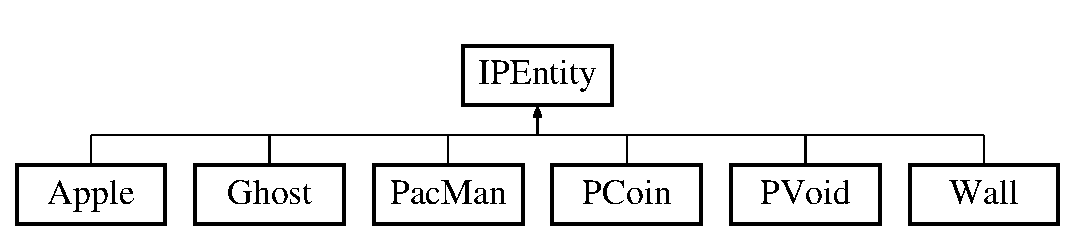
\includegraphics[height=2.000000cm]{class_i_p_entity}
\end{center}
\end{figure}
\subsection*{Public Member Functions}
\begin{DoxyCompactItemize}
\item 
\mbox{\Hypertarget{class_i_p_entity_ac2d45f995beb9a39f117b93e0c87f7a4}\label{class_i_p_entity_ac2d45f995beb9a39f117b93e0c87f7a4}} 
virtual \hyperlink{struct_vector2}{Vector2}$<$ int $>$ {\bfseries get\+Position} ()=0
\item 
\mbox{\Hypertarget{class_i_p_entity_aee49045a3d435ab19ad0f74ca732c347}\label{class_i_p_entity_aee49045a3d435ab19ad0f74ca732c347}} 
virtual std\+::string {\bfseries get\+Name} ()=0
\item 
\mbox{\Hypertarget{class_i_p_entity_a1e205532c04d76b77520e434661c0a52}\label{class_i_p_entity_a1e205532c04d76b77520e434661c0a52}} 
virtual std\+::string {\bfseries get\+Color} ()=0
\end{DoxyCompactItemize}


The documentation for this class was generated from the following file\+:\begin{DoxyCompactItemize}
\item 
games/\+Pac\+Man/I\+Entity.\+hpp\end{DoxyCompactItemize}

\hypertarget{class_launcher}{}\section{Launcher Class Reference}
\label{class_launcher}\index{Launcher@{Launcher}}
\subsection*{Public Member Functions}
\begin{DoxyCompactItemize}
\item 
\hyperlink{class_launcher_a7be10dda45e4e1704c05b6284b60f9c5}{Launcher} ()
\begin{DoxyCompactList}\small\item\em \hyperlink{class_launcher}{Launcher} constructor. \end{DoxyCompactList}\item 
\mbox{\Hypertarget{class_launcher_a4cfd9a0c7ad40c110f9a38662dde5db1}\label{class_launcher_a4cfd9a0c7ad40c110f9a38662dde5db1}} 
const std\+::vector$<$ std\+::string $>$ \& {\bfseries get\+Instructions} (const std\+::string \&event)
\item 
\mbox{\Hypertarget{class_launcher_aba555060beb5382e816709f8a7571c38}\label{class_launcher_aba555060beb5382e816709f8a7571c38}} 
void {\bfseries update\+Index} (const std\+::string \&direction)
\item 
\mbox{\Hypertarget{class_launcher_a875d96b76e44deffa7229c92486db4c7}\label{class_launcher_a875d96b76e44deffa7229c92486db4c7}} 
const std\+::string {\bfseries format\+Text} (const std\+::string \&text) const
\item 
\mbox{\Hypertarget{class_launcher_a403b3f5149cb3b727df45f9ca6b4d1c9}\label{class_launcher_a403b3f5149cb3b727df45f9ca6b4d1c9}} 
const std\+::string {\bfseries get\+Color} (const int \&index) const
\end{DoxyCompactItemize}


\subsection{Constructor \& Destructor Documentation}
\mbox{\Hypertarget{class_launcher_a7be10dda45e4e1704c05b6284b60f9c5}\label{class_launcher_a7be10dda45e4e1704c05b6284b60f9c5}} 
\index{Launcher@{Launcher}!Launcher@{Launcher}}
\index{Launcher@{Launcher}!Launcher@{Launcher}}
\subsubsection{\texorpdfstring{Launcher()}{Launcher()}}
{\footnotesize\ttfamily Launcher\+::\+Launcher (\begin{DoxyParamCaption}{ }\end{DoxyParamCaption})}



\hyperlink{class_launcher}{Launcher} constructor. 

Init \hyperlink{class_launcher}{Launcher} and scan ./games directory to discover \+\_\+\+\_\+.\+so games Games are sorted alphabetically

\begin{DoxyReturn}{Returns}
New instance of \hyperlink{class_launcher}{Launcher} 
\end{DoxyReturn}


The documentation for this class was generated from the following files\+:\begin{DoxyCompactItemize}
\item 
core/Launcher.\+hpp\item 
core/Launcher.\+cpp\end{DoxyCompactItemize}

\hypertarget{class_lib_ncurse}{}\section{Lib\+Ncurse Class Reference}
\label{class_lib_ncurse}\index{Lib\+Ncurse@{Lib\+Ncurse}}
Inheritance diagram for Lib\+Ncurse\+:\begin{figure}[H]
\begin{center}
\leavevmode
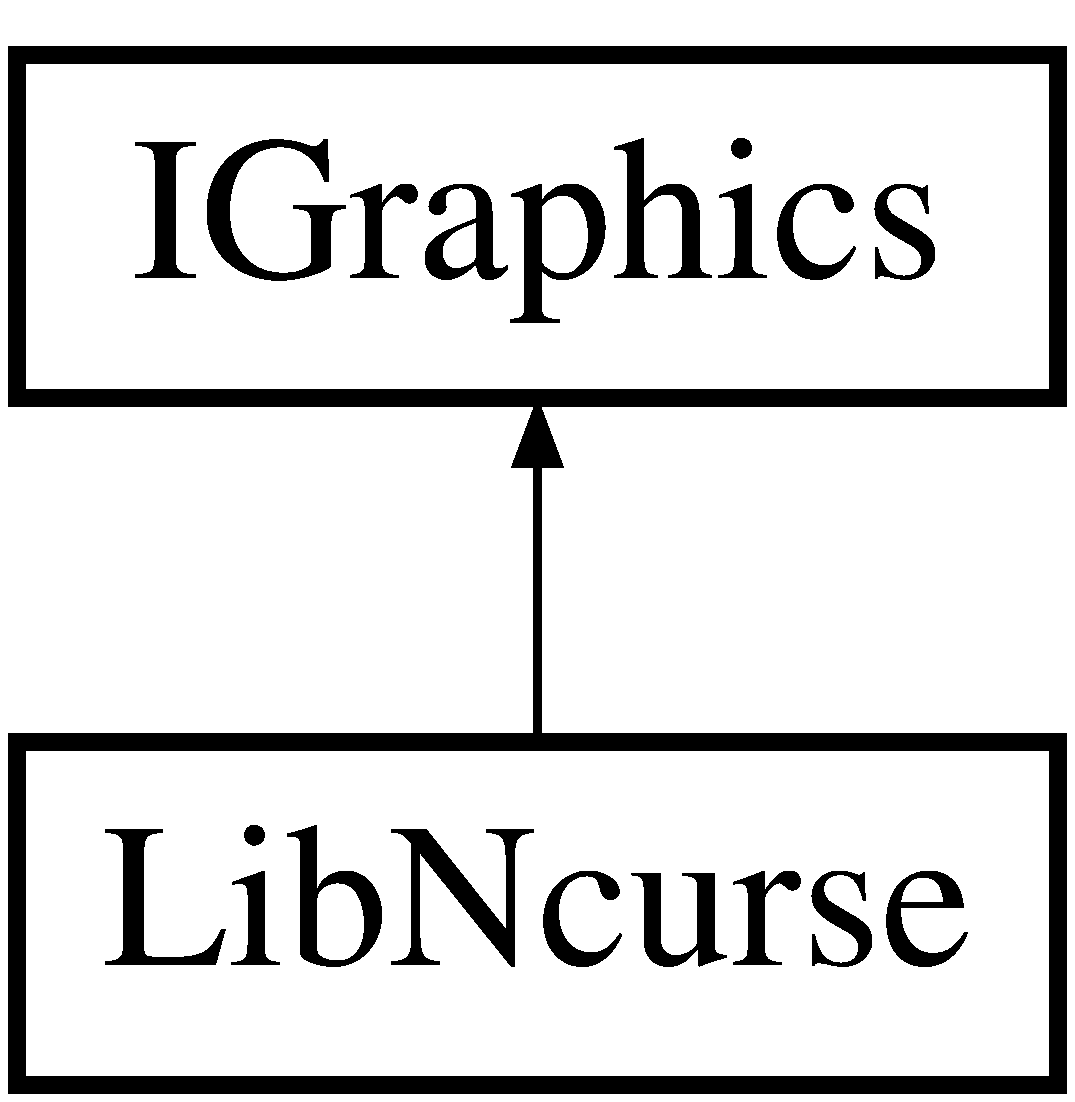
\includegraphics[height=2.000000cm]{class_lib_ncurse}
\end{center}
\end{figure}
\subsection*{Public Member Functions}
\begin{DoxyCompactItemize}
\item 
\mbox{\Hypertarget{class_lib_ncurse_a902000326da1191a5a9ec01f576fefbe}\label{class_lib_ncurse_a902000326da1191a5a9ec01f576fefbe}} 
void {\bfseries Init} ()
\item 
\mbox{\Hypertarget{class_lib_ncurse_a4df45ee61d2979f449f5d76997a6afb4}\label{class_lib_ncurse_a4df45ee61d2979f449f5d76997a6afb4}} 
void {\bfseries draw\+Rectangle} (const \hyperlink{struct_rectangle}{Rectangle}$<$ int $>$ \&rect, const std\+::string \&color) final
\item 
\mbox{\Hypertarget{class_lib_ncurse_a79d59d86d893ccecbf3cd2c17f7ff538}\label{class_lib_ncurse_a79d59d86d893ccecbf3cd2c17f7ff538}} 
void {\bfseries draw\+Window} () final
\item 
\mbox{\Hypertarget{class_lib_ncurse_abb8a827f8529d331dfcb2cae28dc1358}\label{class_lib_ncurse_abb8a827f8529d331dfcb2cae28dc1358}} 
const std\+::string {\bfseries handle\+Event} () final
\item 
\mbox{\Hypertarget{class_lib_ncurse_a612535eaae922d0c42ab3f3ed5ffc10c}\label{class_lib_ncurse_a612535eaae922d0c42ab3f3ed5ffc10c}} 
void {\bfseries load\+Textures} (std\+::vector$<$ std\+::string $>$) final
\item 
\mbox{\Hypertarget{class_lib_ncurse_a75aea5747954e458b997146a5cc83705}\label{class_lib_ncurse_a75aea5747954e458b997146a5cc83705}} 
std\+::string {\bfseries get\+String} ()
\item 
\mbox{\Hypertarget{class_lib_ncurse_af5952c8c4e13f59ac701d91e50e1c7e6}\label{class_lib_ncurse_af5952c8c4e13f59ac701d91e50e1c7e6}} 
void {\bfseries enter\+Text\+Mode} ()
\item 
\mbox{\Hypertarget{class_lib_ncurse_aa587f9bf27b087297bd346da6c8044d1}\label{class_lib_ncurse_aa587f9bf27b087297bd346da6c8044d1}} 
const int {\bfseries get\+Color} (std\+::string) const
\item 
\mbox{\Hypertarget{class_lib_ncurse_aba1b05011ddaf8f889951aecd2908301}\label{class_lib_ncurse_aba1b05011ddaf8f889951aecd2908301}} 
void {\bfseries draw\+Text} (const std\+::string \&str, const \hyperlink{struct_vector2}{Vector2}$<$ int $>$ \&position, const std\+::string \&color) final
\item 
\mbox{\Hypertarget{class_lib_ncurse_a624e99b020c70f610afa53f3435d05d9}\label{class_lib_ncurse_a624e99b020c70f610afa53f3435d05d9}} 
void {\bfseries clear\+Window} () final
\item 
\mbox{\Hypertarget{class_lib_ncurse_aab5802cbe2362f2dac726aafb7035373}\label{class_lib_ncurse_aab5802cbe2362f2dac726aafb7035373}} 
void {\bfseries close} () final
\item 
\mbox{\Hypertarget{class_lib_ncurse_ad3389ed9b5cc782c7dbda5f96cdce2ce}\label{class_lib_ncurse_ad3389ed9b5cc782c7dbda5f96cdce2ce}} 
const bool {\bfseries is\+Open} () const final
\end{DoxyCompactItemize}


The documentation for this class was generated from the following files\+:\begin{DoxyCompactItemize}
\item 
lib/ncurses/Lib\+Ncurse.\+hpp\item 
lib/ncurses/Lib\+Ncurse.\+cpp\end{DoxyCompactItemize}

\hypertarget{class_lib_open_g_l}{}\section{Lib\+Open\+GL Class Reference}
\label{class_lib_open_g_l}\index{Lib\+Open\+GL@{Lib\+Open\+GL}}
Inheritance diagram for Lib\+Open\+GL\+:\begin{figure}[H]
\begin{center}
\leavevmode
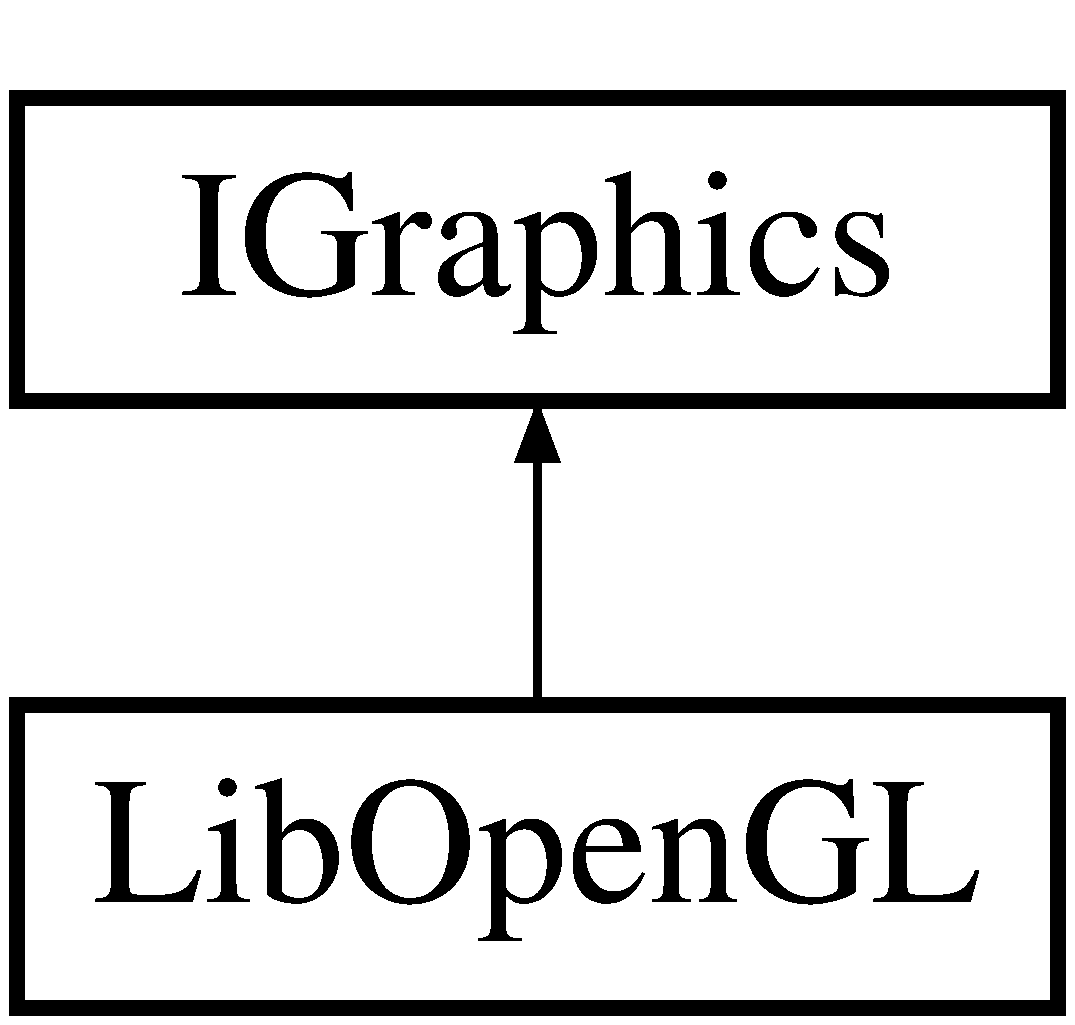
\includegraphics[height=2.000000cm]{class_lib_open_g_l}
\end{center}
\end{figure}
\subsection*{Public Member Functions}
\begin{DoxyCompactItemize}
\item 
\mbox{\Hypertarget{class_lib_open_g_l_a12fec3fecead61d7d796d614a636923e}\label{class_lib_open_g_l_a12fec3fecead61d7d796d614a636923e}} 
void {\bfseries Init} ()
\item 
\mbox{\Hypertarget{class_lib_open_g_l_af9b43e06e5b0f06f7e5949bf64ad10cc}\label{class_lib_open_g_l_af9b43e06e5b0f06f7e5949bf64ad10cc}} 
void {\bfseries draw\+Rectangle} (const \hyperlink{struct_rectangle}{Rectangle}$<$ int $>$ \&rect, const std\+::string \&color) final
\item 
\mbox{\Hypertarget{class_lib_open_g_l_a76706c1c8659644160411a712d963156}\label{class_lib_open_g_l_a76706c1c8659644160411a712d963156}} 
void {\bfseries draw\+Window} () final
\item 
\mbox{\Hypertarget{class_lib_open_g_l_a9a4701c7cd4560d911c5610e9f155f97}\label{class_lib_open_g_l_a9a4701c7cd4560d911c5610e9f155f97}} 
const std\+::string {\bfseries handle\+Event} () final
\item 
\mbox{\Hypertarget{class_lib_open_g_l_a2846434326ea029ec1a33768ac9d4c0b}\label{class_lib_open_g_l_a2846434326ea029ec1a33768ac9d4c0b}} 
void {\bfseries load\+Textures} (std\+::vector$<$ std\+::string $>$) final
\item 
\mbox{\Hypertarget{class_lib_open_g_l_ad5d671d5aa8227245b58b82470ce80c2}\label{class_lib_open_g_l_ad5d671d5aa8227245b58b82470ce80c2}} 
sf\+::\+Color {\bfseries get\+Color} (std\+::string) const
\item 
\mbox{\Hypertarget{class_lib_open_g_l_adbc38936d3ca931c0402b070b00bb26f}\label{class_lib_open_g_l_adbc38936d3ca931c0402b070b00bb26f}} 
void {\bfseries enter\+Text\+Mode} (void)
\item 
\mbox{\Hypertarget{class_lib_open_g_l_af22247b140bc426eb4794bc9857e09b5}\label{class_lib_open_g_l_af22247b140bc426eb4794bc9857e09b5}} 
void {\bfseries draw\+Text} (const std\+::string \&str, const \hyperlink{struct_vector2}{Vector2}$<$ int $>$ \&position, const std\+::string \&color) final
\item 
\mbox{\Hypertarget{class_lib_open_g_l_a47bb8a26e010dde8cefa71e30872bb2b}\label{class_lib_open_g_l_a47bb8a26e010dde8cefa71e30872bb2b}} 
void {\bfseries clear\+Window} () final
\item 
\mbox{\Hypertarget{class_lib_open_g_l_a3e3809b6dd1d0cd50eea2893448ffa01}\label{class_lib_open_g_l_a3e3809b6dd1d0cd50eea2893448ffa01}} 
void {\bfseries close} () final
\item 
\mbox{\Hypertarget{class_lib_open_g_l_aa4243545ecc1f17a06e0fc05d645cd37}\label{class_lib_open_g_l_aa4243545ecc1f17a06e0fc05d645cd37}} 
const bool {\bfseries is\+Open} () const final
\end{DoxyCompactItemize}


The documentation for this class was generated from the following files\+:\begin{DoxyCompactItemize}
\item 
lib/\+Open\+G\+L/Lib\+Open\+G\+L.\+hpp\item 
lib/\+Open\+G\+L/Lib\+Open\+G\+L.\+cpp\end{DoxyCompactItemize}

\hypertarget{class_lib_s_f_m_l}{}\section{Lib\+S\+F\+ML Class Reference}
\label{class_lib_s_f_m_l}\index{Lib\+S\+F\+ML@{Lib\+S\+F\+ML}}
Inheritance diagram for Lib\+S\+F\+ML\+:\begin{figure}[H]
\begin{center}
\leavevmode
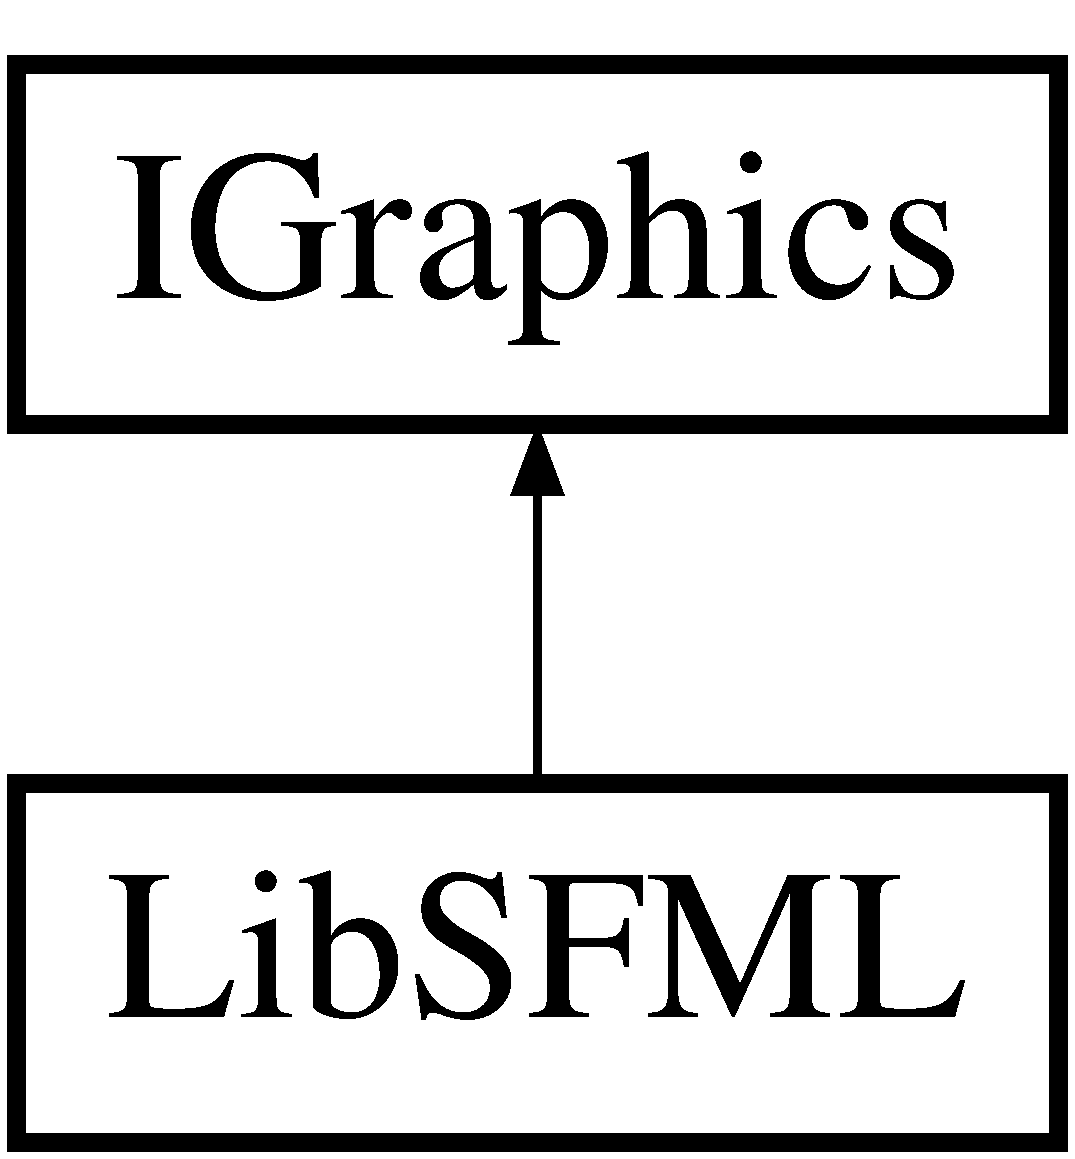
\includegraphics[height=2.000000cm]{class_lib_s_f_m_l}
\end{center}
\end{figure}
\subsection*{Public Member Functions}
\begin{DoxyCompactItemize}
\item 
\mbox{\Hypertarget{class_lib_s_f_m_l_a33fd692ece121874840da35d56d3df4e}\label{class_lib_s_f_m_l_a33fd692ece121874840da35d56d3df4e}} 
void {\bfseries Init} ()
\item 
\mbox{\Hypertarget{class_lib_s_f_m_l_ab1a5d951083dfc702e79f726cdc5d02f}\label{class_lib_s_f_m_l_ab1a5d951083dfc702e79f726cdc5d02f}} 
void {\bfseries draw\+Rectangle} (const \hyperlink{struct_rectangle}{Rectangle}$<$ int $>$ \&rect, const std\+::string \&color) final
\item 
\mbox{\Hypertarget{class_lib_s_f_m_l_a1e1977ccb48ae960e01768fed04839d8}\label{class_lib_s_f_m_l_a1e1977ccb48ae960e01768fed04839d8}} 
void {\bfseries draw\+Window} () final
\item 
\mbox{\Hypertarget{class_lib_s_f_m_l_ad049067dedb7f127e36381c7416a4b9a}\label{class_lib_s_f_m_l_ad049067dedb7f127e36381c7416a4b9a}} 
const std\+::string {\bfseries handle\+Event} () final
\item 
\mbox{\Hypertarget{class_lib_s_f_m_l_a0c7f8e6d9cd4f5d6582fa4130cf2ef6d}\label{class_lib_s_f_m_l_a0c7f8e6d9cd4f5d6582fa4130cf2ef6d}} 
void {\bfseries load\+Textures} (std\+::vector$<$ std\+::string $>$) final
\item 
\mbox{\Hypertarget{class_lib_s_f_m_l_af24977140de7d20472a1508263f99b47}\label{class_lib_s_f_m_l_af24977140de7d20472a1508263f99b47}} 
void {\bfseries enter\+Text\+Mode} ()
\item 
\mbox{\Hypertarget{class_lib_s_f_m_l_a7b03cdce04f1f38abadb8b7499c758f9}\label{class_lib_s_f_m_l_a7b03cdce04f1f38abadb8b7499c758f9}} 
sf\+::\+Color {\bfseries get\+Color} (std\+::string) const
\item 
\mbox{\Hypertarget{class_lib_s_f_m_l_ad6f9617cc719daf16da0f339155c83c1}\label{class_lib_s_f_m_l_ad6f9617cc719daf16da0f339155c83c1}} 
void {\bfseries draw\+Text} (const std\+::string \&str, const \hyperlink{struct_vector2}{Vector2}$<$ int $>$ \&position, const std\+::string \&color) final
\item 
\mbox{\Hypertarget{class_lib_s_f_m_l_a82143915dd2ff04fecdd0eadc78f8cdd}\label{class_lib_s_f_m_l_a82143915dd2ff04fecdd0eadc78f8cdd}} 
void {\bfseries clear\+Window} () final
\item 
\mbox{\Hypertarget{class_lib_s_f_m_l_ad1439ed141a3c01620edbb4188392027}\label{class_lib_s_f_m_l_ad1439ed141a3c01620edbb4188392027}} 
void {\bfseries close} () final
\item 
\mbox{\Hypertarget{class_lib_s_f_m_l_a7343eab898faa0e2ac2a0e0d867b400f}\label{class_lib_s_f_m_l_a7343eab898faa0e2ac2a0e0d867b400f}} 
const bool {\bfseries is\+Open} () const final
\end{DoxyCompactItemize}


The documentation for this class was generated from the following files\+:\begin{DoxyCompactItemize}
\item 
lib/\+S\+F\+M\+L/Lib\+S\+F\+M\+L.\+hpp\item 
lib/\+S\+F\+M\+L/Lib\+S\+F\+M\+L.\+cpp\end{DoxyCompactItemize}

\hypertarget{class_manager}{}\section{Manager Class Reference}
\label{class_manager}\index{Manager@{Manager}}
\subsection*{Public Member Functions}
\begin{DoxyCompactItemize}
\item 
\hyperlink{class_manager_a72554004e4ab55571d9907455de28656}{Manager} (const std\+::string \&default\+Lib)
\begin{DoxyCompactList}\small\item\em \hyperlink{class_manager}{Manager} constructor. \end{DoxyCompactList}\item 
\mbox{\Hypertarget{class_manager_a15d49cb59cbcd720e172ee0c6259e7d0}\label{class_manager_a15d49cb59cbcd720e172ee0c6259e7d0}} 
void {\bfseries Change\+Library} (const std\+::string \&)
\item 
\mbox{\Hypertarget{class_manager_aac988fe1a7a4cca17c0933d4ae5fffb4}\label{class_manager_aac988fe1a7a4cca17c0933d4ae5fffb4}} 
void \hyperlink{class_manager_aac988fe1a7a4cca17c0933d4ae5fffb4}{Execute\+Instructions} (void)
\begin{DoxyCompactList}\small\item\em Execute game\textquotesingle{}s instruction Get instruction from the game, parse and execute. \end{DoxyCompactList}\item 
\mbox{\Hypertarget{class_manager_aeaea2e0414fef6b4bede43e7c9680840}\label{class_manager_aeaea2e0414fef6b4bede43e7c9680840}} 
void \hyperlink{class_manager_aeaea2e0414fef6b4bede43e7c9680840}{Load\+Textures} (void)
\begin{DoxyCompactList}\small\item\em Load texures of the loaded game. \end{DoxyCompactList}\item 
\hyperlink{class_i_graphics}{I\+Graphics} \& \hyperlink{class_manager_a8cb265f0bd19351a88df4c167ece1377}{Get\+Instance} (void)
\begin{DoxyCompactList}\small\item\em Get the instance of the current graphical library. \end{DoxyCompactList}\item 
\mbox{\Hypertarget{class_manager_a38a6ba7243dc9aa08922d77509141f8e}\label{class_manager_a38a6ba7243dc9aa08922d77509141f8e}} 
void {\bfseries update\+Score} (std\+::string score)
\end{DoxyCompactItemize}


\subsection{Constructor \& Destructor Documentation}
\mbox{\Hypertarget{class_manager_a72554004e4ab55571d9907455de28656}\label{class_manager_a72554004e4ab55571d9907455de28656}} 
\index{Manager@{Manager}!Manager@{Manager}}
\index{Manager@{Manager}!Manager@{Manager}}
\subsubsection{\texorpdfstring{Manager()}{Manager()}}
{\footnotesize\ttfamily Manager\+::\+Manager (\begin{DoxyParamCaption}\item[{const std\+::string \&}]{default\+Lib }\end{DoxyParamCaption})}



\hyperlink{class_manager}{Manager} constructor. 

Initialize core manager. Load all graphical libraries from lib/ folder Initialize the \begin{DoxyParagraph}{default\+Lib}

\end{DoxyParagraph}
\begin{DoxyReturn}{Returns}
New instance of \hyperlink{class_manager}{Manager} 
\end{DoxyReturn}


\subsection{Member Function Documentation}
\mbox{\Hypertarget{class_manager_a8cb265f0bd19351a88df4c167ece1377}\label{class_manager_a8cb265f0bd19351a88df4c167ece1377}} 
\index{Manager@{Manager}!Get\+Instance@{Get\+Instance}}
\index{Get\+Instance@{Get\+Instance}!Manager@{Manager}}
\subsubsection{\texorpdfstring{Get\+Instance()}{GetInstance()}}
{\footnotesize\ttfamily \hyperlink{class_i_graphics}{I\+Graphics} \& Manager\+::\+Get\+Instance (\begin{DoxyParamCaption}\item[{void}]{ }\end{DoxyParamCaption})}



Get the instance of the current graphical library. 

If {\ttfamily \hyperlink{class_manager_a8cb265f0bd19351a88df4c167ece1377}{Get\+Instance()}} from \hyperlink{class_d_l_loader}{D\+L\+Loader} fail, an \hyperlink{class_arcade_exception}{Arcade\+Exception} is thrown and the program exit.

\begin{DoxyReturn}{Returns}
A reference to a graphical library 
\end{DoxyReturn}


The documentation for this class was generated from the following files\+:\begin{DoxyCompactItemize}
\item 
core/\+D\+L\+Loader/Manager.\+hpp\item 
core/\+D\+L\+Loader/Manager.\+cpp\end{DoxyCompactItemize}

\hypertarget{class_object}{}\section{Object Class Reference}
\label{class_object}\index{Object@{Object}}
Inheritance diagram for Object\+:\begin{figure}[H]
\begin{center}
\leavevmode
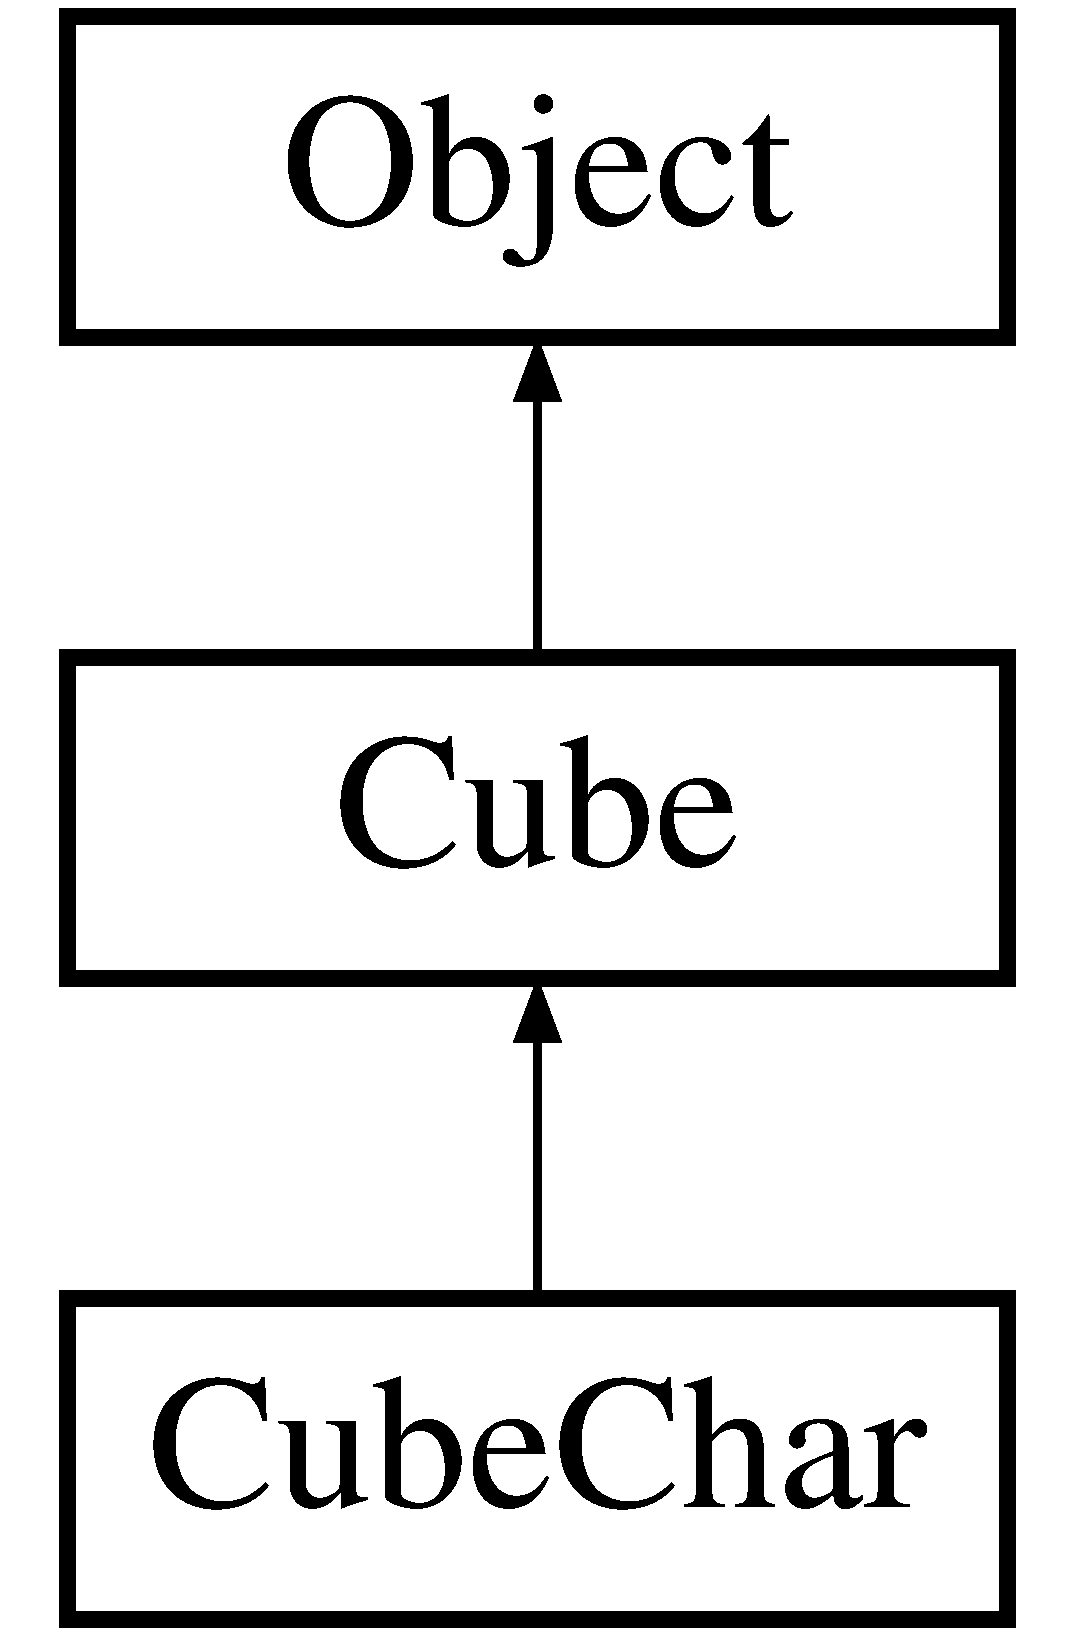
\includegraphics[height=3.000000cm]{class_object}
\end{center}
\end{figure}
\subsection*{Public Types}
\begin{DoxyCompactItemize}
\item 
\mbox{\Hypertarget{class_object_a9bb8746e3c466dae7df7f8745e548b41}\label{class_object_a9bb8746e3c466dae7df7f8745e548b41}} 
enum {\bfseries Cam\+Enum} \{ \newline
{\bfseries P\+O\+S\+\_\+X}, 
{\bfseries P\+O\+S\+\_\+Y}, 
{\bfseries P\+O\+S\+\_\+Z}, 
{\bfseries R\+O\+T\+\_\+X}, 
\newline
{\bfseries R\+O\+T\+\_\+Y}, 
{\bfseries R\+O\+T\+\_\+Z}, 
{\bfseries S\+C\+A\+L\+E\+\_\+X}, 
{\bfseries S\+C\+A\+L\+E\+\_\+Y}, 
\newline
{\bfseries S\+C\+A\+L\+E\+\_\+Z}
 \}
\end{DoxyCompactItemize}
\subsection*{Public Member Functions}
\begin{DoxyCompactItemize}
\item 
\mbox{\Hypertarget{class_object_a762153e3524db0b2eb74dbe71a346320}\label{class_object_a762153e3524db0b2eb74dbe71a346320}} 
{\bfseries Object} (const glm\+::vec3 \&position=glm\+::vec3(0.\+0f, 0.\+0f, 0.\+0f), const glm\+::vec3 \&rotation=glm\+::vec3(0.\+0f, 0.\+0f, 0.\+0f), const glm\+::vec3 \&scalation=glm\+::vec3(1.\+0f, 1.\+0f, 1.\+0f))
\item 
\mbox{\Hypertarget{class_object_accca66b4eaf6fabfcc30335b5b61c2b0}\label{class_object_accca66b4eaf6fabfcc30335b5b61c2b0}} 
void {\bfseries set\+V\+BO} (const uint \&vbo, const uint \&vertice\+Nb)
\item 
\mbox{\Hypertarget{class_object_a146f845664b3c1597fc38f9ec96e213a}\label{class_object_a146f845664b3c1597fc38f9ec96e213a}} 
void {\bfseries set\+E\+BO} (const uint \&ebo, const uint \&indice\+Nb)
\item 
\mbox{\Hypertarget{class_object_a9fdaca6f7c488ab33ac13e87bd592c73}\label{class_object_a9fdaca6f7c488ab33ac13e87bd592c73}} 
void {\bfseries set\+V\+AO} (const uint \&vao)
\item 
\mbox{\Hypertarget{class_object_a8fd0f444323745a0e2ac7d93a5bfebd8}\label{class_object_a8fd0f444323745a0e2ac7d93a5bfebd8}} 
uint {\bfseries get\+V\+BO} (void) const
\item 
\mbox{\Hypertarget{class_object_aac91fcf10fe0becb8951b135c93c566a}\label{class_object_aac91fcf10fe0becb8951b135c93c566a}} 
uint {\bfseries get\+E\+BO} (void) const
\item 
\mbox{\Hypertarget{class_object_abb81a00502ed4444ac27bb3851bfee8a}\label{class_object_abb81a00502ed4444ac27bb3851bfee8a}} 
uint {\bfseries get\+V\+AO} (void) const
\item 
\mbox{\Hypertarget{class_object_ab0bb4f22fd1dbf20a2ae8c6755b683a3}\label{class_object_ab0bb4f22fd1dbf20a2ae8c6755b683a3}} 
const \hyperlink{class_shader}{Shader} \& {\bfseries get\+Shader} (void)
\item 
\mbox{\Hypertarget{class_object_a6af4ee5d88817a5d136a64c6b1601a18}\label{class_object_a6af4ee5d88817a5d136a64c6b1601a18}} 
void {\bfseries set\+Vertices} (const float $\ast$array, uint array\+Size, G\+Lenum draw\+Type)
\item 
\mbox{\Hypertarget{class_object_a57a89e83099e91a5e33316dfdc37bd95}\label{class_object_a57a89e83099e91a5e33316dfdc37bd95}} 
void {\bfseries set\+Vertices} (const std\+::vector$<$ float $>$ \&array, G\+Lenum draw\+Type)
\item 
\mbox{\Hypertarget{class_object_a84e6b296710f817596fa8ff7ad09d6ef}\label{class_object_a84e6b296710f817596fa8ff7ad09d6ef}} 
void {\bfseries set\+Indices} (const uint $\ast$array, uint array\+Size, G\+Lenum draw\+Type)
\item 
\mbox{\Hypertarget{class_object_a93b4e7330b5ccf3355fd53e202f5127c}\label{class_object_a93b4e7330b5ccf3355fd53e202f5127c}} 
void {\bfseries set\+Indices} (const std\+::vector$<$ uint $>$ \&array, G\+Lenum draw\+Type)
\item 
\mbox{\Hypertarget{class_object_ace74c7c5c63465778a46208f3f8aa708}\label{class_object_ace74c7c5c63465778a46208f3f8aa708}} 
void {\bfseries set\+Shader} (const \hyperlink{class_shader}{Shader} \&shader, const glm\+::mat4 \&projection\+Matrix)
\item 
\mbox{\Hypertarget{class_object_af1040cb216f7ca9db4c9578438949765}\label{class_object_af1040cb216f7ca9db4c9578438949765}} 
void {\bfseries set\+Texture} (std\+::shared\+\_\+ptr$<$ \hyperlink{class_texture}{Texture} $>$ texture)
\item 
\mbox{\Hypertarget{class_object_a15a01f840e0d23dcb531dc3e11db48c8}\label{class_object_a15a01f840e0d23dcb531dc3e11db48c8}} 
void {\bfseries draw} (G\+Lenum draw\+Mode, const glm\+::mat4 \&projection\+Matrix, const \hyperlink{class_camera}{Camera} \&c)
\item 
\mbox{\Hypertarget{class_object_ac9ec1252fbc5ed5f0e939327c49502df}\label{class_object_ac9ec1252fbc5ed5f0e939327c49502df}} 
void {\bfseries set\+View\+Matrix} (const glm\+::mat4 \&view\+Matrix)
\item 
\mbox{\Hypertarget{class_object_add03115634ae6d9b2e7b3f60b7e18fb7}\label{class_object_add03115634ae6d9b2e7b3f60b7e18fb7}} 
void {\bfseries set\+Translate} (void)
\item 
\mbox{\Hypertarget{class_object_a47499992846ea51d38c619ed8198692d}\label{class_object_a47499992846ea51d38c619ed8198692d}} 
void {\bfseries set\+Scale} (void)
\item 
\mbox{\Hypertarget{class_object_ae938828b5b801c7240f960612355eb0f}\label{class_object_ae938828b5b801c7240f960612355eb0f}} 
void {\bfseries set\+Rotate} (void)
\item 
\mbox{\Hypertarget{class_object_a05e1a120de109beb5bdd57dd137b1689}\label{class_object_a05e1a120de109beb5bdd57dd137b1689}} 
void {\bfseries set\+Position} (const glm\+::vec3 \&position)
\item 
\mbox{\Hypertarget{class_object_a5211444ea1b8e56ad9d6727d00c69f33}\label{class_object_a5211444ea1b8e56ad9d6727d00c69f33}} 
void {\bfseries set\+Scalation} (const glm\+::vec3 \&scalation)
\item 
\mbox{\Hypertarget{class_object_aea32ce3191fdae2dd8d89573a0bbc829}\label{class_object_aea32ce3191fdae2dd8d89573a0bbc829}} 
void {\bfseries set\+Rotation} (const glm\+::vec3 \&rotation)
\item 
\mbox{\Hypertarget{class_object_ad0f8e3212f78eede8a6bca2177154b72}\label{class_object_ad0f8e3212f78eede8a6bca2177154b72}} 
void {\bfseries move} (const Cam\+Enum \&axe, const float \&distance)
\item 
\mbox{\Hypertarget{class_object_ad88f29fe3f7e8cf661156291c1a7f607}\label{class_object_ad88f29fe3f7e8cf661156291c1a7f607}} 
void {\bfseries scale} (const Cam\+Enum \&axe, const float \&strength)
\item 
\mbox{\Hypertarget{class_object_a14e4e02ae69334c12bfab9cb47703a02}\label{class_object_a14e4e02ae69334c12bfab9cb47703a02}} 
void {\bfseries rotate} (const Cam\+Enum \&axe, const float \&degrees)
\item 
\mbox{\Hypertarget{class_object_a1688d829b96ed8374dbc619b47b5dfcc}\label{class_object_a1688d829b96ed8374dbc619b47b5dfcc}} 
void {\bfseries actualize\+Transform} (const glm\+::mat4 \&projection\+Matrix)
\end{DoxyCompactItemize}


The documentation for this class was generated from the following files\+:\begin{DoxyCompactItemize}
\item 
lib/\+Open\+G\+L/classes/Object.\+hpp\item 
lib/\+Open\+G\+L/classes/Object.\+cpp\end{DoxyCompactItemize}

\hypertarget{class_pac_man}{}\section{Pac\+Man Class Reference}
\label{class_pac_man}\index{Pac\+Man@{Pac\+Man}}
Inheritance diagram for Pac\+Man\+:\begin{figure}[H]
\begin{center}
\leavevmode
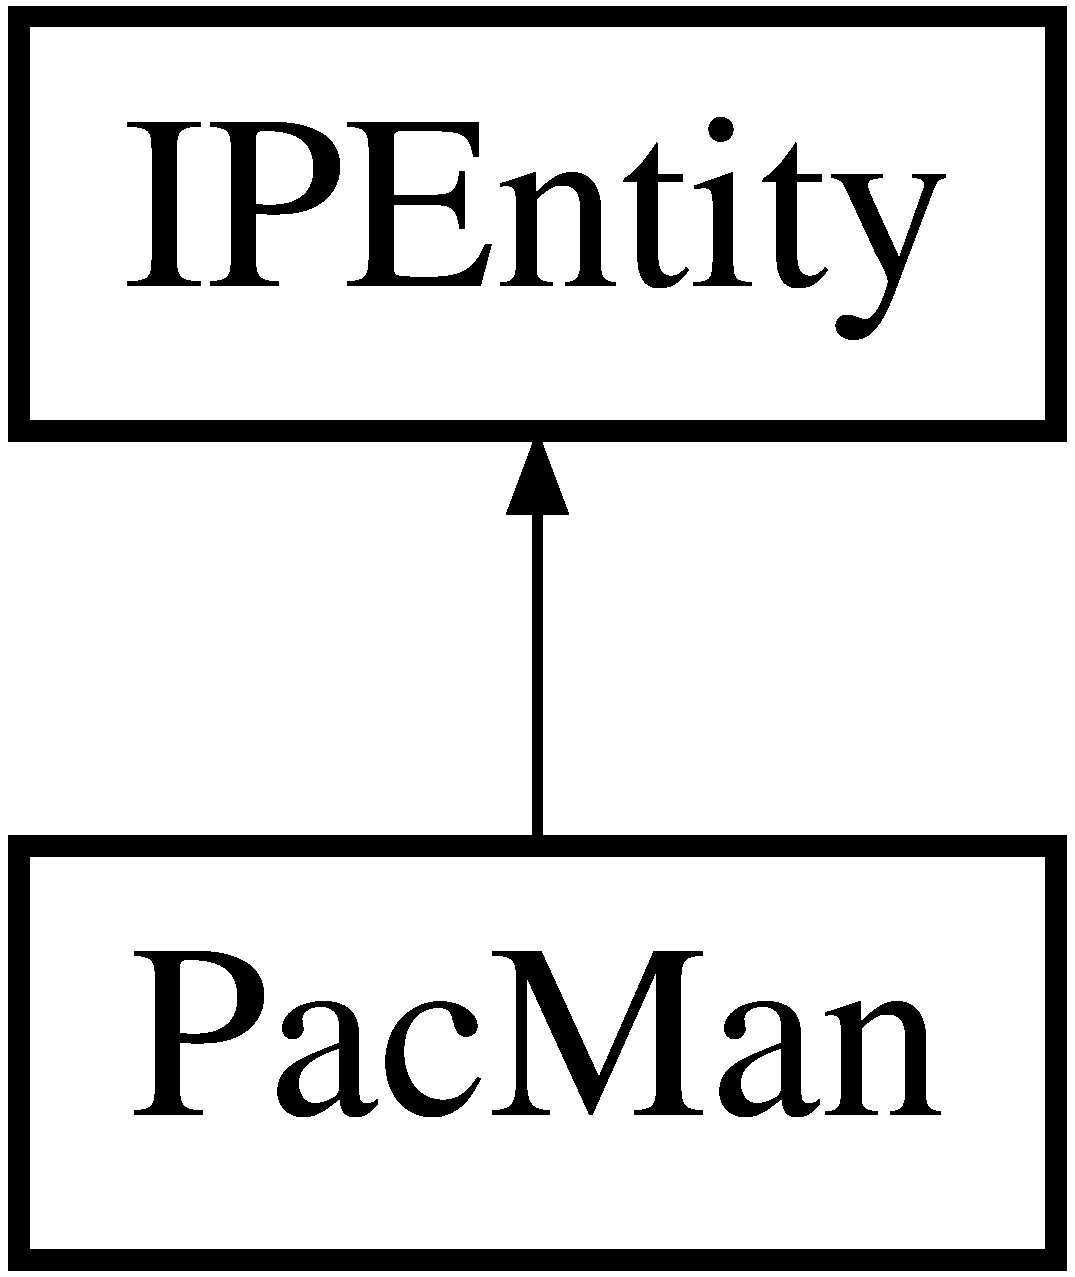
\includegraphics[height=2.000000cm]{class_pac_man}
\end{center}
\end{figure}
\subsection*{Public Member Functions}
\begin{DoxyCompactItemize}
\item 
\mbox{\Hypertarget{class_pac_man_a5ab6b0be0c7d80e35832d886d9c22789}\label{class_pac_man_a5ab6b0be0c7d80e35832d886d9c22789}} 
{\bfseries Pac\+Man} (\hyperlink{struct_vector2}{Vector2}$<$ int $>$ pos, \hyperlink{struct_vector2}{Vector2}$<$ int $>$ dir)
\item 
\mbox{\Hypertarget{class_pac_man_a3c7a9c5a76023a8c710c18d1d2b5ff5f}\label{class_pac_man_a3c7a9c5a76023a8c710c18d1d2b5ff5f}} 
\hyperlink{struct_vector2}{Vector2}$<$ int $>$ {\bfseries get\+Position} ()
\item 
\mbox{\Hypertarget{class_pac_man_a9300c86d9704b60f1efdaa015134877c}\label{class_pac_man_a9300c86d9704b60f1efdaa015134877c}} 
\hyperlink{struct_vector2}{Vector2}$<$ int $>$ {\bfseries get\+Dir} ()
\item 
\mbox{\Hypertarget{class_pac_man_a6271bcaed94b99d95e0188213704dada}\label{class_pac_man_a6271bcaed94b99d95e0188213704dada}} 
std\+::string {\bfseries get\+Name} ()
\item 
\mbox{\Hypertarget{class_pac_man_aada56f8c4de59a0be1d1041bb561074f}\label{class_pac_man_aada56f8c4de59a0be1d1041bb561074f}} 
void {\bfseries set\+Pos} (\hyperlink{struct_vector2}{Vector2}$<$ int $>$)
\item 
\mbox{\Hypertarget{class_pac_man_ae7395e5123f61e0f10106314baabd569}\label{class_pac_man_ae7395e5123f61e0f10106314baabd569}} 
std\+::string {\bfseries get\+Color} ()
\item 
\mbox{\Hypertarget{class_pac_man_aeba4de62a1b7999054e290b5a84812b2}\label{class_pac_man_aeba4de62a1b7999054e290b5a84812b2}} 
void {\bfseries move} ()
\item 
\mbox{\Hypertarget{class_pac_man_a2f6d02ec46957070b966c24b816d93dd}\label{class_pac_man_a2f6d02ec46957070b966c24b816d93dd}} 
void {\bfseries set\+Dir} (\hyperlink{struct_vector2}{Vector2}$<$ int $>$)
\end{DoxyCompactItemize}


The documentation for this class was generated from the following files\+:\begin{DoxyCompactItemize}
\item 
games/\+Pac\+Man/Pac\+Man.\+hpp\item 
games/\+Pac\+Man/Pac\+Man.\+cpp\end{DoxyCompactItemize}

\hypertarget{class_pac_man_scene}{}\section{Pac\+Man\+Scene Class Reference}
\label{class_pac_man_scene}\index{Pac\+Man\+Scene@{Pac\+Man\+Scene}}
Inheritance diagram for Pac\+Man\+Scene\+:\begin{figure}[H]
\begin{center}
\leavevmode
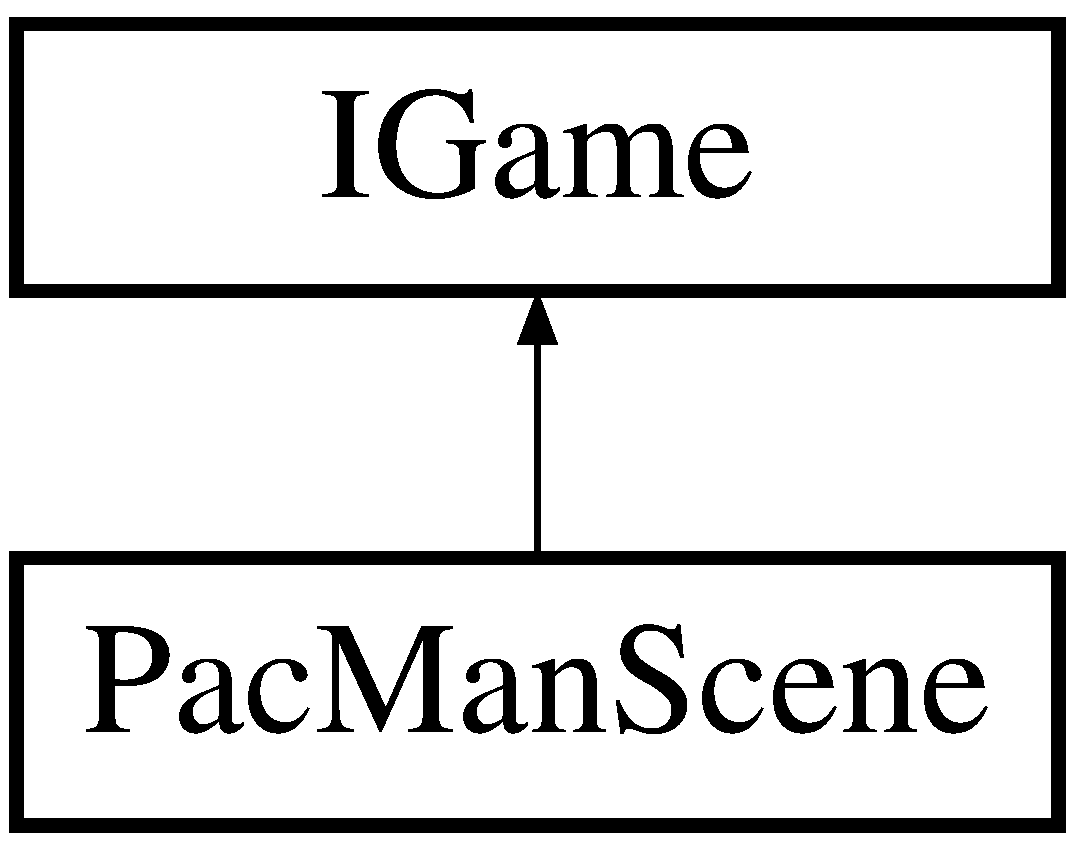
\includegraphics[height=2.000000cm]{class_pac_man_scene}
\end{center}
\end{figure}
\subsection*{Public Member Functions}
\begin{DoxyCompactItemize}
\item 
\mbox{\Hypertarget{class_pac_man_scene_aed1cba4fdcc5de835eaad230b7f91c7a}\label{class_pac_man_scene_aed1cba4fdcc5de835eaad230b7f91c7a}} 
void {\bfseries update} (const std\+::string \&input) final
\item 
\mbox{\Hypertarget{class_pac_man_scene_a36aa174f984c0d95f7640d202d8e7147}\label{class_pac_man_scene_a36aa174f984c0d95f7640d202d8e7147}} 
void {\bfseries update\+Board} ()
\item 
\mbox{\Hypertarget{class_pac_man_scene_a44afe54e906f4e52399885170c60fd54}\label{class_pac_man_scene_a44afe54e906f4e52399885170c60fd54}} 
void {\bfseries check\+Apple} ()
\item 
\mbox{\Hypertarget{class_pac_man_scene_a18907fcbd5b997b1c189eeff16ad976a}\label{class_pac_man_scene_a18907fcbd5b997b1c189eeff16ad976a}} 
void {\bfseries check\+Ghost} ()
\item 
\mbox{\Hypertarget{class_pac_man_scene_a227a7de2f0bb9c20f983d450695a2b51}\label{class_pac_man_scene_a227a7de2f0bb9c20f983d450695a2b51}} 
void {\bfseries check\+Coin} ()
\item 
\mbox{\Hypertarget{class_pac_man_scene_a822b15e261ac1fd601b7b9807529cbff}\label{class_pac_man_scene_a822b15e261ac1fd601b7b9807529cbff}} 
void {\bfseries check\+Wall} (\hyperlink{struct_vector2}{Vector2}$<$ int $>$ old\+Pos, \hyperlink{struct_vector2}{Vector2}$<$ int $>$ old\+Dir)
\item 
\mbox{\Hypertarget{class_pac_man_scene_a3a4ac446de6df34415b202530884469e}\label{class_pac_man_scene_a3a4ac446de6df34415b202530884469e}} 
void {\bfseries draw\+Board} (std\+::vector$<$ std\+::string $>$ \&)
\item 
\mbox{\Hypertarget{class_pac_man_scene_a75698a31bbe77a495277c7fa64ca5f94}\label{class_pac_man_scene_a75698a31bbe77a495277c7fa64ca5f94}} 
void {\bfseries fill\+Coin} ()
\item 
\mbox{\Hypertarget{class_pac_man_scene_a1bab9f4bac4f6369b124b4387eeda097}\label{class_pac_man_scene_a1bab9f4bac4f6369b124b4387eeda097}} 
std\+::vector$<$ std\+::string $>$ {\bfseries Send\+Instruction} () final
\item 
\mbox{\Hypertarget{class_pac_man_scene_a53d3395cbcdd4192aab8aacf751f79d0}\label{class_pac_man_scene_a53d3395cbcdd4192aab8aacf751f79d0}} 
std\+::string {\bfseries get\+Name} ()
\item 
\mbox{\Hypertarget{class_pac_man_scene_a343de23273852ce28dbac16bac963ebc}\label{class_pac_man_scene_a343de23273852ce28dbac16bac963ebc}} 
std\+::vector$<$ std\+::string $>$ {\bfseries get\+Textures} () final
\item 
\mbox{\Hypertarget{class_pac_man_scene_a68f11fa508813abe9872a3b618287d2d}\label{class_pac_man_scene_a68f11fa508813abe9872a3b618287d2d}} 
void {\bfseries move\+\_\+ghosts} ()
\end{DoxyCompactItemize}


The documentation for this class was generated from the following files\+:\begin{DoxyCompactItemize}
\item 
games/\+Pac\+Man/Pac\+Man\+Scene.\+hpp\item 
games/\+Pac\+Man/Pac\+Man\+Scene.\+cpp\end{DoxyCompactItemize}

\hypertarget{class_p_coin}{}\section{P\+Coin Class Reference}
\label{class_p_coin}\index{P\+Coin@{P\+Coin}}
Inheritance diagram for P\+Coin\+:\begin{figure}[H]
\begin{center}
\leavevmode
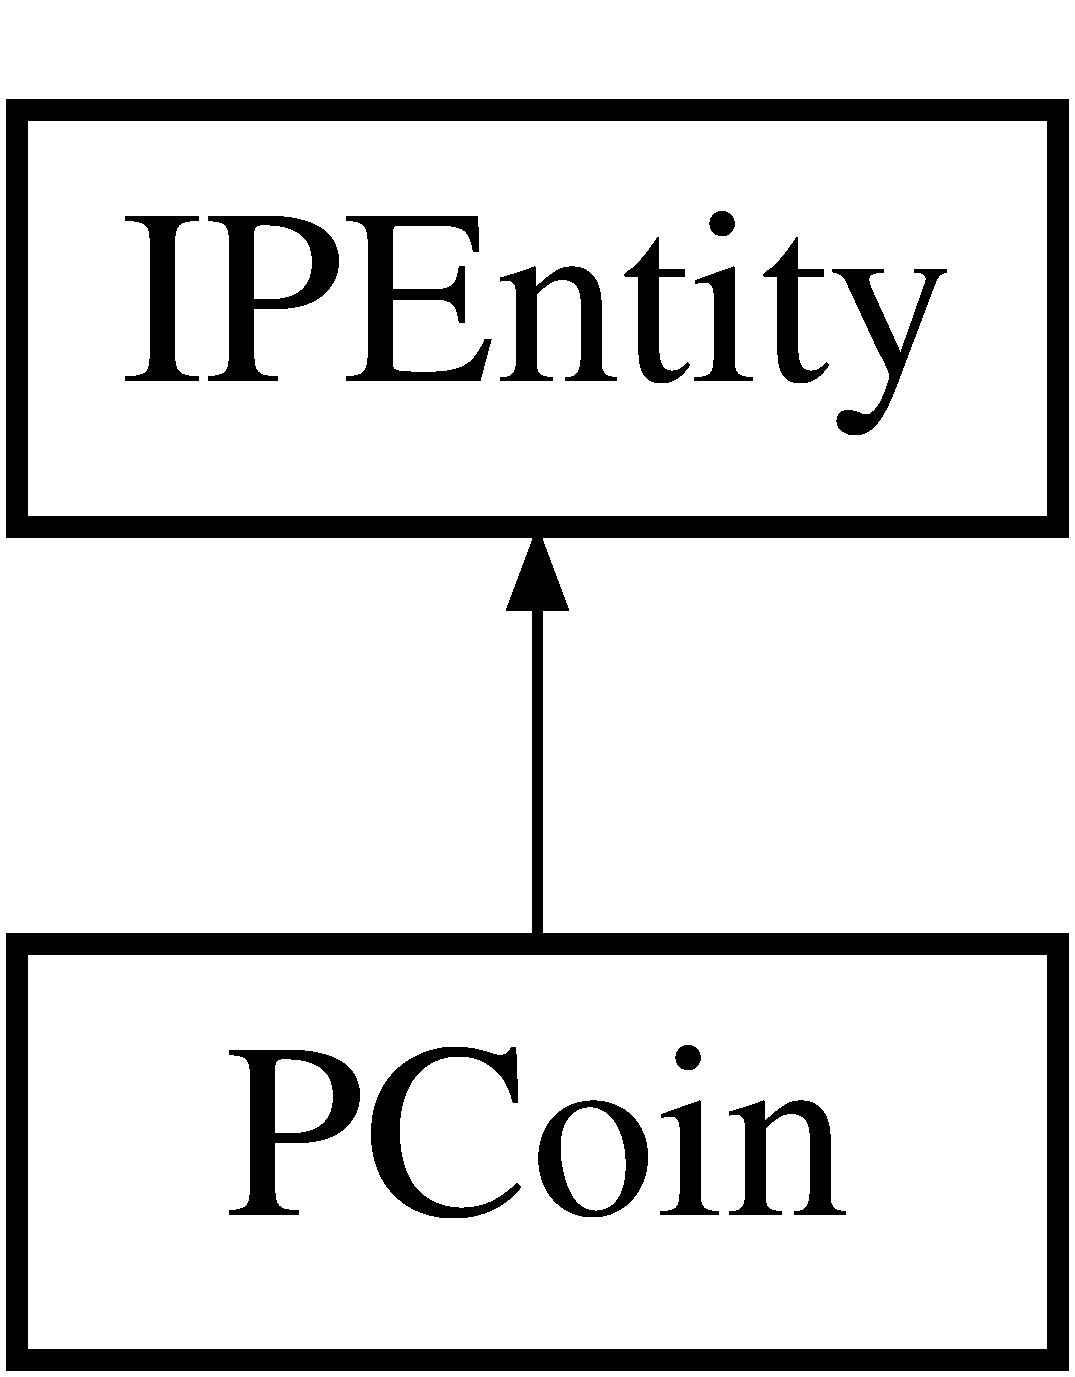
\includegraphics[height=2.000000cm]{class_p_coin}
\end{center}
\end{figure}
\subsection*{Public Member Functions}
\begin{DoxyCompactItemize}
\item 
\mbox{\Hypertarget{class_p_coin_ade72369af211c6301b9ce19d3949e3f7}\label{class_p_coin_ade72369af211c6301b9ce19d3949e3f7}} 
{\bfseries P\+Coin} (\hyperlink{struct_vector2}{Vector2}$<$ int $>$ pos)
\item 
\mbox{\Hypertarget{class_p_coin_a929ca2a7bc64e2593ff48542e1a97737}\label{class_p_coin_a929ca2a7bc64e2593ff48542e1a97737}} 
\hyperlink{struct_vector2}{Vector2}$<$ int $>$ {\bfseries get\+Position} ()
\item 
\mbox{\Hypertarget{class_p_coin_a1fcb17fdcc1579c4a377afeab7fc65ac}\label{class_p_coin_a1fcb17fdcc1579c4a377afeab7fc65ac}} 
std\+::string {\bfseries get\+Name} ()
\item 
\mbox{\Hypertarget{class_p_coin_a5855ef970021bac99481b87a94304335}\label{class_p_coin_a5855ef970021bac99481b87a94304335}} 
std\+::string {\bfseries get\+Color} ()
\end{DoxyCompactItemize}


The documentation for this class was generated from the following files\+:\begin{DoxyCompactItemize}
\item 
games/\+Pac\+Man/Coin.\+hpp\item 
games/\+Pac\+Man/Coin.\+cpp\end{DoxyCompactItemize}

\hypertarget{class_p_void}{}\section{P\+Void Class Reference}
\label{class_p_void}\index{P\+Void@{P\+Void}}
Inheritance diagram for P\+Void\+:\begin{figure}[H]
\begin{center}
\leavevmode
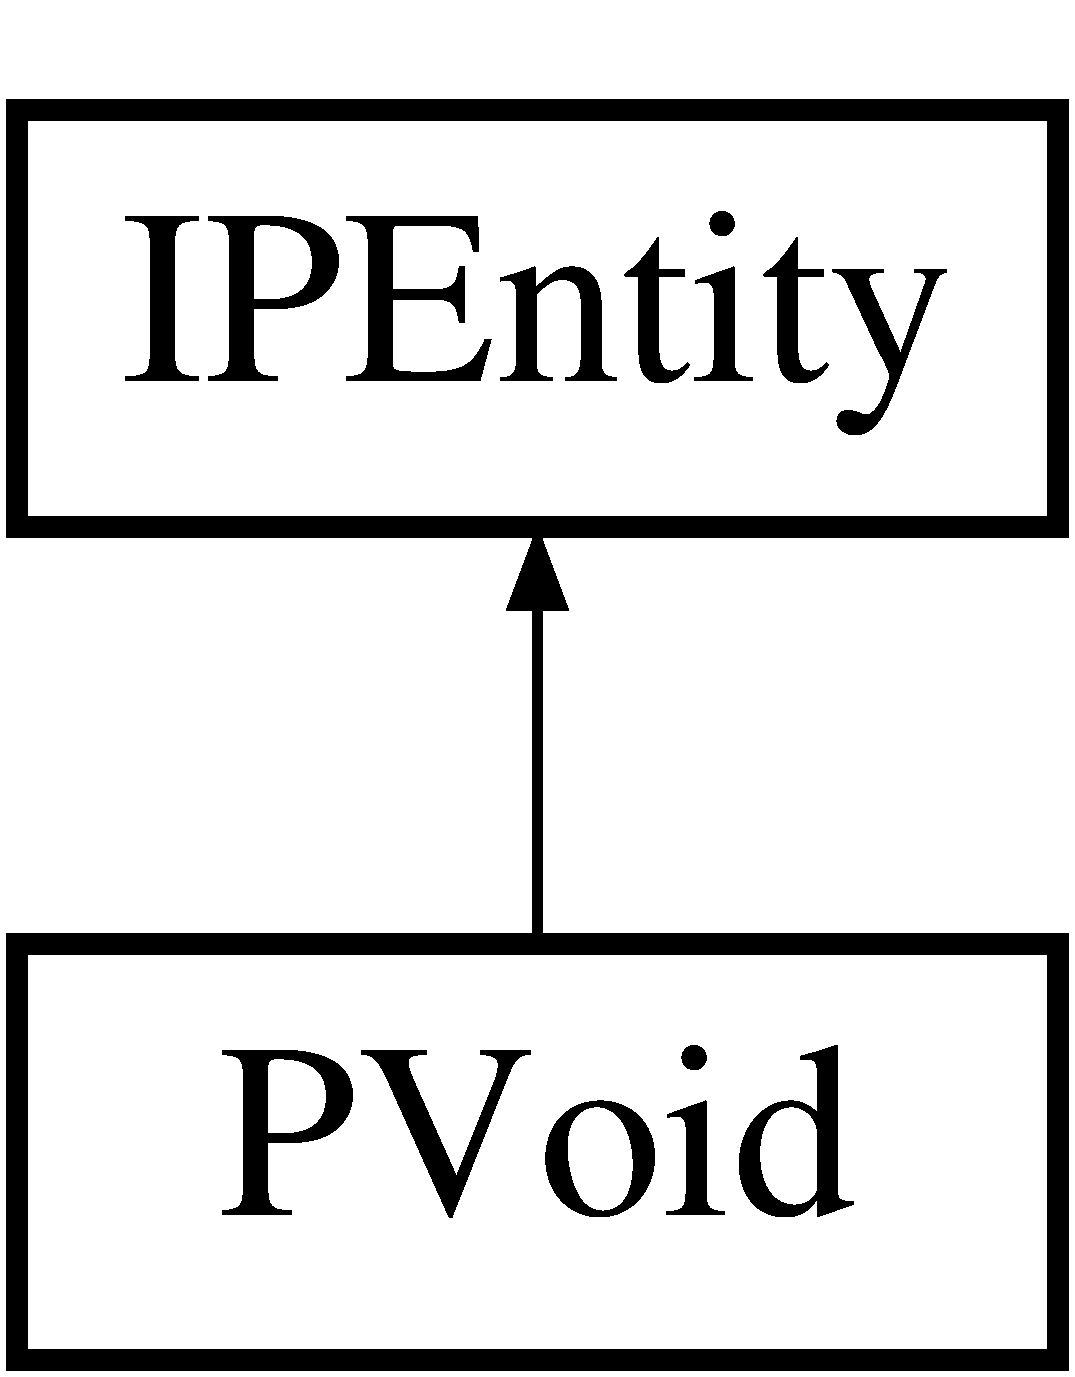
\includegraphics[height=2.000000cm]{class_p_void}
\end{center}
\end{figure}
\subsection*{Public Member Functions}
\begin{DoxyCompactItemize}
\item 
\mbox{\Hypertarget{class_p_void_aca093f464068d1c4a0d15998f3d9f716}\label{class_p_void_aca093f464068d1c4a0d15998f3d9f716}} 
std\+::string {\bfseries get\+Name} () final
\item 
\mbox{\Hypertarget{class_p_void_a7ce40aadd2847d9ff110fe5103a1c53d}\label{class_p_void_a7ce40aadd2847d9ff110fe5103a1c53d}} 
std\+::string {\bfseries get\+Color} () final
\item 
\mbox{\Hypertarget{class_p_void_aa887ea58e955bee9ff19328d75109776}\label{class_p_void_aa887ea58e955bee9ff19328d75109776}} 
\hyperlink{struct_vector2}{Vector2}$<$ int $>$ {\bfseries get\+Position} ()
\end{DoxyCompactItemize}


The documentation for this class was generated from the following files\+:\begin{DoxyCompactItemize}
\item 
games/\+Pac\+Man/P\+Void.\+hpp\item 
games/\+Pac\+Man/P\+Void.\+cpp\end{DoxyCompactItemize}

\hypertarget{struct_rectangle}{}\section{Rectangle$<$ T $>$ Struct Template Reference}
\label{struct_rectangle}\index{Rectangle$<$ T $>$@{Rectangle$<$ T $>$}}
\subsection*{Public Member Functions}
\begin{DoxyCompactItemize}
\item 
\mbox{\Hypertarget{struct_rectangle_af8e17300c0d03bc93c7e1b5e6e969a80}\label{struct_rectangle_af8e17300c0d03bc93c7e1b5e6e969a80}} 
{\bfseries Rectangle} (const T \&\+\_\+p1, const T \&\+\_\+p2, const T \&\+\_\+p3, const T \&\+\_\+p4)
\item 
\mbox{\Hypertarget{struct_rectangle_aaefc1e19dacbca8f4672bfe3bd449c98}\label{struct_rectangle_aaefc1e19dacbca8f4672bfe3bd449c98}} 
void {\bfseries Set\+Position} (const T \&\+\_\+p1, const T \&\+\_\+p2, const T \&\+\_\+p3, const T \&\+\_\+p4)
\end{DoxyCompactItemize}
\subsection*{Public Attributes}
\begin{DoxyCompactItemize}
\item 
\mbox{\Hypertarget{struct_rectangle_aacd2b0c397b8df1e3df2fa93516d7dac}\label{struct_rectangle_aacd2b0c397b8df1e3df2fa93516d7dac}} 
T {\bfseries p1}
\item 
\mbox{\Hypertarget{struct_rectangle_adb4391197618708e3ee812eadc0a3365}\label{struct_rectangle_adb4391197618708e3ee812eadc0a3365}} 
T {\bfseries p2}
\item 
\mbox{\Hypertarget{struct_rectangle_af056110dc4403bcad6ab43ba679d6d8c}\label{struct_rectangle_af056110dc4403bcad6ab43ba679d6d8c}} 
T {\bfseries p3}
\item 
\mbox{\Hypertarget{struct_rectangle_adb507bf1b5ad378d45fd96e2fc3cd81f}\label{struct_rectangle_adb507bf1b5ad378d45fd96e2fc3cd81f}} 
T {\bfseries p4}
\end{DoxyCompactItemize}


The documentation for this struct was generated from the following file\+:\begin{DoxyCompactItemize}
\item 
lib/\+Templates/Rectangle.\+hpp\end{DoxyCompactItemize}

\hypertarget{class_shader}{}\section{Shader Class Reference}
\label{class_shader}\index{Shader@{Shader}}
\subsection*{Public Member Functions}
\begin{DoxyCompactItemize}
\item 
\mbox{\Hypertarget{class_shader_a0a40ea1ce78aa2d3ea16e4be7374a341}\label{class_shader_a0a40ea1ce78aa2d3ea16e4be7374a341}} 
{\bfseries Shader} (const std\+::string \&vert\+File, const std\+::string \&frag\+File)
\item 
\mbox{\Hypertarget{class_shader_a8c6d7a517434745f2a68f08c33747c76}\label{class_shader_a8c6d7a517434745f2a68f08c33747c76}} 
const bool {\bfseries set\+Shader} (const std\+::string \&file, const G\+Lenum \&type)
\item 
\mbox{\Hypertarget{class_shader_a36f9ff713f9e50f4d09891d47dc3812c}\label{class_shader_a36f9ff713f9e50f4d09891d47dc3812c}} 
void {\bfseries set\+Uniform\+Bool} (const std\+::string \&name, const bool \&value) const
\item 
\mbox{\Hypertarget{class_shader_af302034f8393f45d2f6957ac7f948689}\label{class_shader_af302034f8393f45d2f6957ac7f948689}} 
void {\bfseries set\+Uniform\+Int} (const std\+::string \&name, const int \&value) const
\item 
\mbox{\Hypertarget{class_shader_a6036a5e3036bc7d6926f1d019b0cb489}\label{class_shader_a6036a5e3036bc7d6926f1d019b0cb489}} 
void {\bfseries set\+Uniform\+Float} (const std\+::string \&name, const float \&value) const
\item 
\mbox{\Hypertarget{class_shader_a18d3289ec71bd0e1bf6b8b4f3776eb7e}\label{class_shader_a18d3289ec71bd0e1bf6b8b4f3776eb7e}} 
void {\bfseries set\+Mat4} (const std\+::string \&name, const glm\+::mat4 \&vals)
\item 
\mbox{\Hypertarget{class_shader_a35543033bad31acc9104947b07c49ec1}\label{class_shader_a35543033bad31acc9104947b07c49ec1}} 
const bool {\bfseries link\+Shader\+Program} (void)
\item 
\mbox{\Hypertarget{class_shader_aca3b1c42d29e6cc7225a49bc652063b0}\label{class_shader_aca3b1c42d29e6cc7225a49bc652063b0}} 
void {\bfseries reset} (void)
\item 
\mbox{\Hypertarget{class_shader_a02e8d41d27aa2b4f229bc6ea681a6521}\label{class_shader_a02e8d41d27aa2b4f229bc6ea681a6521}} 
void {\bfseries use\+Program} (void) const
\item 
\mbox{\Hypertarget{class_shader_ab4dcb37eabe7c84587570a47206b0899}\label{class_shader_ab4dcb37eabe7c84587570a47206b0899}} 
G\+Luint {\bfseries get\+Program\+Id} (void) const
\end{DoxyCompactItemize}


The documentation for this class was generated from the following files\+:\begin{DoxyCompactItemize}
\item 
lib/\+Open\+G\+L/classes/Shader.\+hpp\item 
lib/\+Open\+G\+L/classes/Shader.\+cpp\end{DoxyCompactItemize}

\hypertarget{class_snake}{}\section{Snake Class Reference}
\label{class_snake}\index{Snake@{Snake}}
Inheritance diagram for Snake\+:\begin{figure}[H]
\begin{center}
\leavevmode
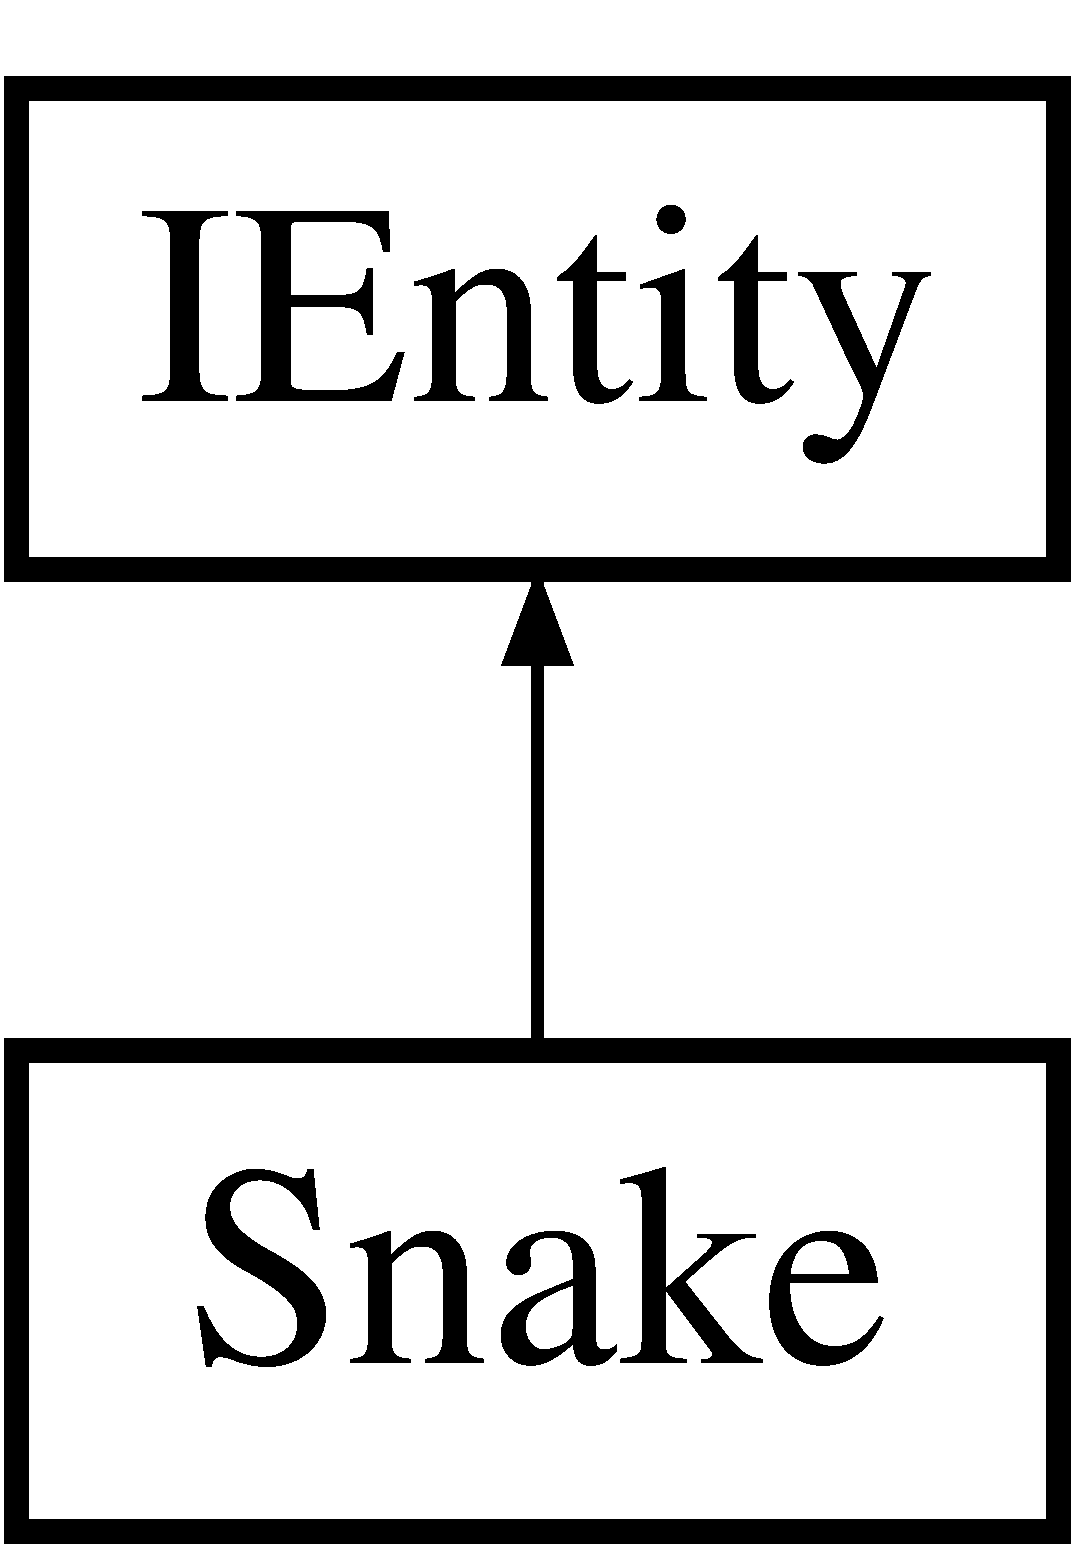
\includegraphics[height=2.000000cm]{class_snake}
\end{center}
\end{figure}
\subsection*{Public Member Functions}
\begin{DoxyCompactItemize}
\item 
\mbox{\Hypertarget{class_snake_a8b14a5c95a9b8106099bde83661e155e}\label{class_snake_a8b14a5c95a9b8106099bde83661e155e}} 
{\bfseries Snake} (\hyperlink{struct_vector2}{Vector2}$<$ int $>$, \hyperlink{struct_vector2}{Vector2}$<$ int $>$)
\item 
\mbox{\Hypertarget{class_snake_acf2312330dfcba505eb0bec22356ab7b}\label{class_snake_acf2312330dfcba505eb0bec22356ab7b}} 
std\+::string {\bfseries get\+Name} () final
\item 
\mbox{\Hypertarget{class_snake_a0fce62d24714f5b27ad923beaf29c513}\label{class_snake_a0fce62d24714f5b27ad923beaf29c513}} 
\hyperlink{struct_vector2}{Vector2}$<$ int $>$ {\bfseries get\+Pos} ()
\item 
\mbox{\Hypertarget{class_snake_aaa3246451a2e7ff9f2674c640fd54391}\label{class_snake_aaa3246451a2e7ff9f2674c640fd54391}} 
void {\bfseries unset\+Head} ()
\item 
\mbox{\Hypertarget{class_snake_a84c432b662c23261d889a36708522d57}\label{class_snake_a84c432b662c23261d889a36708522d57}} 
std\+::string {\bfseries get\+Color} () final
\end{DoxyCompactItemize}


The documentation for this class was generated from the following files\+:\begin{DoxyCompactItemize}
\item 
games/\+Snake/Snake.\+hpp\item 
games/\+Snake/Snake.\+cpp\end{DoxyCompactItemize}

\hypertarget{class_snake_scene}{}\section{Snake\+Scene Class Reference}
\label{class_snake_scene}\index{Snake\+Scene@{Snake\+Scene}}
Inheritance diagram for Snake\+Scene\+:\begin{figure}[H]
\begin{center}
\leavevmode
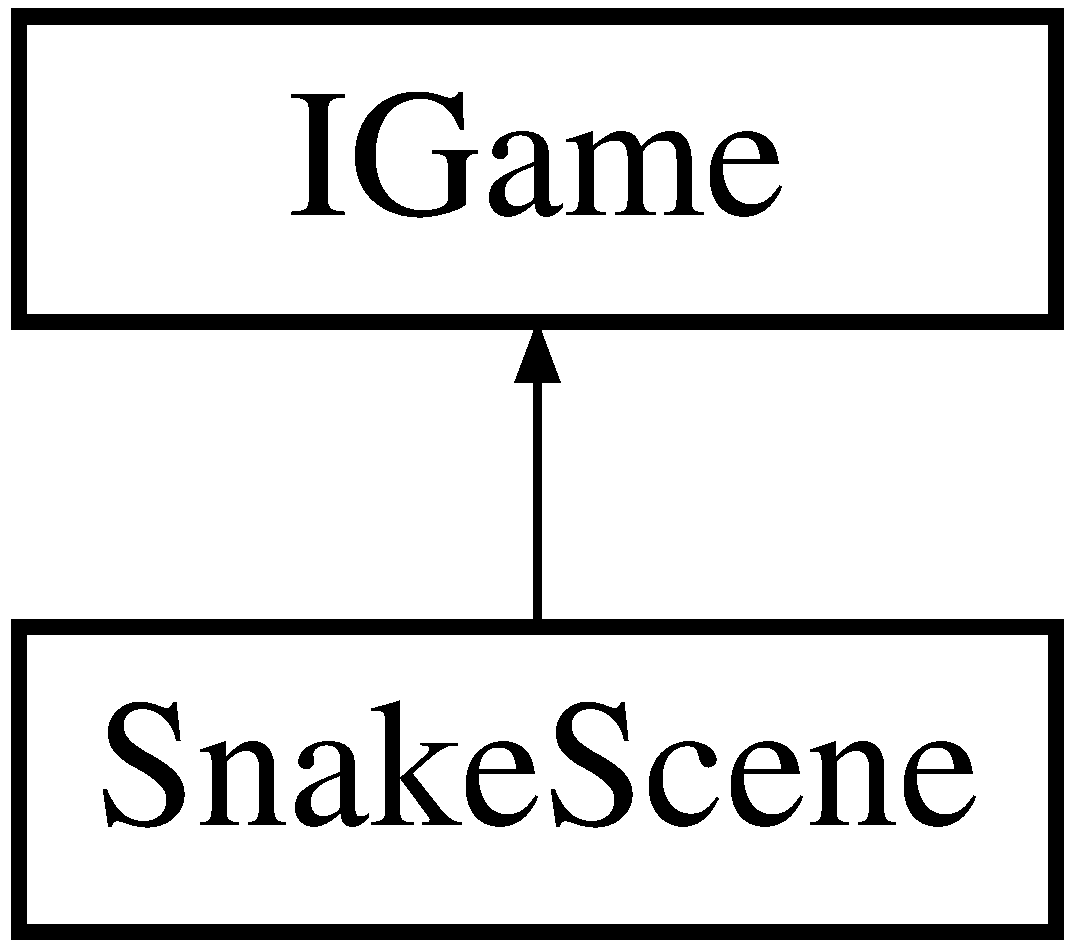
\includegraphics[height=2.000000cm]{class_snake_scene}
\end{center}
\end{figure}
\subsection*{Public Member Functions}
\begin{DoxyCompactItemize}
\item 
\mbox{\Hypertarget{class_snake_scene_af43a25f1cde6abc3afed8c54ac22d235}\label{class_snake_scene_af43a25f1cde6abc3afed8c54ac22d235}} 
void {\bfseries update} (const std\+::string \&input) final
\item 
\mbox{\Hypertarget{class_snake_scene_a84d8f1a9181ab8332469ae564c2145e8}\label{class_snake_scene_a84d8f1a9181ab8332469ae564c2145e8}} 
void {\bfseries update\+Snake\+Pos} ()
\item 
\mbox{\Hypertarget{class_snake_scene_a41b14152eb3e5df7672fe1bb4ad36c38}\label{class_snake_scene_a41b14152eb3e5df7672fe1bb4ad36c38}} 
void {\bfseries Draw\+Board} (std\+::vector$<$ std\+::string $>$ \&instruction) const
\item 
\mbox{\Hypertarget{class_snake_scene_ab88cd1b9a95407dc0e41f23ebc937e89}\label{class_snake_scene_ab88cd1b9a95407dc0e41f23ebc937e89}} 
std\+::vector$<$ std\+::string $>$ {\bfseries Send\+Instruction} () final
\item 
\mbox{\Hypertarget{class_snake_scene_a5847a39fe44c47250e6a8f0be0641d8c}\label{class_snake_scene_a5847a39fe44c47250e6a8f0be0641d8c}} 
std\+::vector$<$ std\+::string $>$ {\bfseries get\+Textures} () final
\item 
\mbox{\Hypertarget{class_snake_scene_a06bd9d46a276bd6f2f92f67ede48152c}\label{class_snake_scene_a06bd9d46a276bd6f2f92f67ede48152c}} 
std\+::string {\bfseries get\+Name} ()
\item 
\mbox{\Hypertarget{class_snake_scene_ac92bd4ff297c2909718cdc229e7b49f3}\label{class_snake_scene_ac92bd4ff297c2909718cdc229e7b49f3}} 
void {\bfseries grow\+Snake} (std\+::vector$<$ std\+::shared\+\_\+ptr$<$ \hyperlink{class_snake}{Snake} $>$ $>$ \&new\+\_\+snake, \hyperlink{struct_vector2}{Vector2}$<$ int $>$ new\+\_\+pos)
\end{DoxyCompactItemize}


The documentation for this class was generated from the following files\+:\begin{DoxyCompactItemize}
\item 
games/\+Snake/Snake\+Scene.\+hpp\item 
games/\+Snake/Snake\+Scene.\+cpp\end{DoxyCompactItemize}

\hypertarget{class_texture}{}\section{Texture Class Reference}
\label{class_texture}\index{Texture@{Texture}}
\subsection*{Public Member Functions}
\begin{DoxyCompactItemize}
\item 
\mbox{\Hypertarget{class_texture_a4cd45e8898c02b5a5c790a479233124b}\label{class_texture_a4cd45e8898c02b5a5c790a479233124b}} 
{\bfseries Texture} (const std\+::string \&path)
\item 
\mbox{\Hypertarget{class_texture_ad25b3ba440143db990376651423aa6da}\label{class_texture_ad25b3ba440143db990376651423aa6da}} 
const uint \& {\bfseries get\+Texture\+Id} (void) const
\item 
\mbox{\Hypertarget{class_texture_a7da06a9a7eb132c4d0dd3ab27ed5e7b1}\label{class_texture_a7da06a9a7eb132c4d0dd3ab27ed5e7b1}} 
const bool {\bfseries load\+Texture} (const std\+::string \&path)
\item 
\mbox{\Hypertarget{class_texture_a81a4d9ab416ccc078c489536a16e0d12}\label{class_texture_a81a4d9ab416ccc078c489536a16e0d12}} 
void {\bfseries bind\+Texture} (void) const
\end{DoxyCompactItemize}


The documentation for this class was generated from the following files\+:\begin{DoxyCompactItemize}
\item 
lib/\+Open\+G\+L/classes/Texture.\+hpp\item 
lib/\+Open\+G\+L/classes/Texture.\+cpp\end{DoxyCompactItemize}

\hypertarget{struct_vector2}{}\section{Vector2$<$ T $>$ Struct Template Reference}
\label{struct_vector2}\index{Vector2$<$ T $>$@{Vector2$<$ T $>$}}
\subsection*{Public Member Functions}
\begin{DoxyCompactItemize}
\item 
\mbox{\Hypertarget{struct_vector2_ab8cf9f67f03bae6dbc56de251fcbee28}\label{struct_vector2_ab8cf9f67f03bae6dbc56de251fcbee28}} 
{\bfseries Vector2} (const T \&\+\_\+x, const T \&\+\_\+y)
\item 
\mbox{\Hypertarget{struct_vector2_a14813c3593ca20eb25c5d7cc1ad6daa4}\label{struct_vector2_a14813c3593ca20eb25c5d7cc1ad6daa4}} 
void {\bfseries Set\+Position} (const T \&\+\_\+x, const T \&\+\_\+y)
\end{DoxyCompactItemize}
\subsection*{Public Attributes}
\begin{DoxyCompactItemize}
\item 
\mbox{\Hypertarget{struct_vector2_a78fa1f2ed5e261c7fbeb8f3536a1ee34}\label{struct_vector2_a78fa1f2ed5e261c7fbeb8f3536a1ee34}} 
T {\bfseries x}
\item 
\mbox{\Hypertarget{struct_vector2_a6cfed8355591aa269f4dba43bd806ef9}\label{struct_vector2_a6cfed8355591aa269f4dba43bd806ef9}} 
T {\bfseries y}
\end{DoxyCompactItemize}


The documentation for this struct was generated from the following file\+:\begin{DoxyCompactItemize}
\item 
lib/\+Templates/Vector.\+hpp\end{DoxyCompactItemize}

\hypertarget{class_void}{}\section{Void Class Reference}
\label{class_void}\index{Void@{Void}}
Inheritance diagram for Void\+:\begin{figure}[H]
\begin{center}
\leavevmode
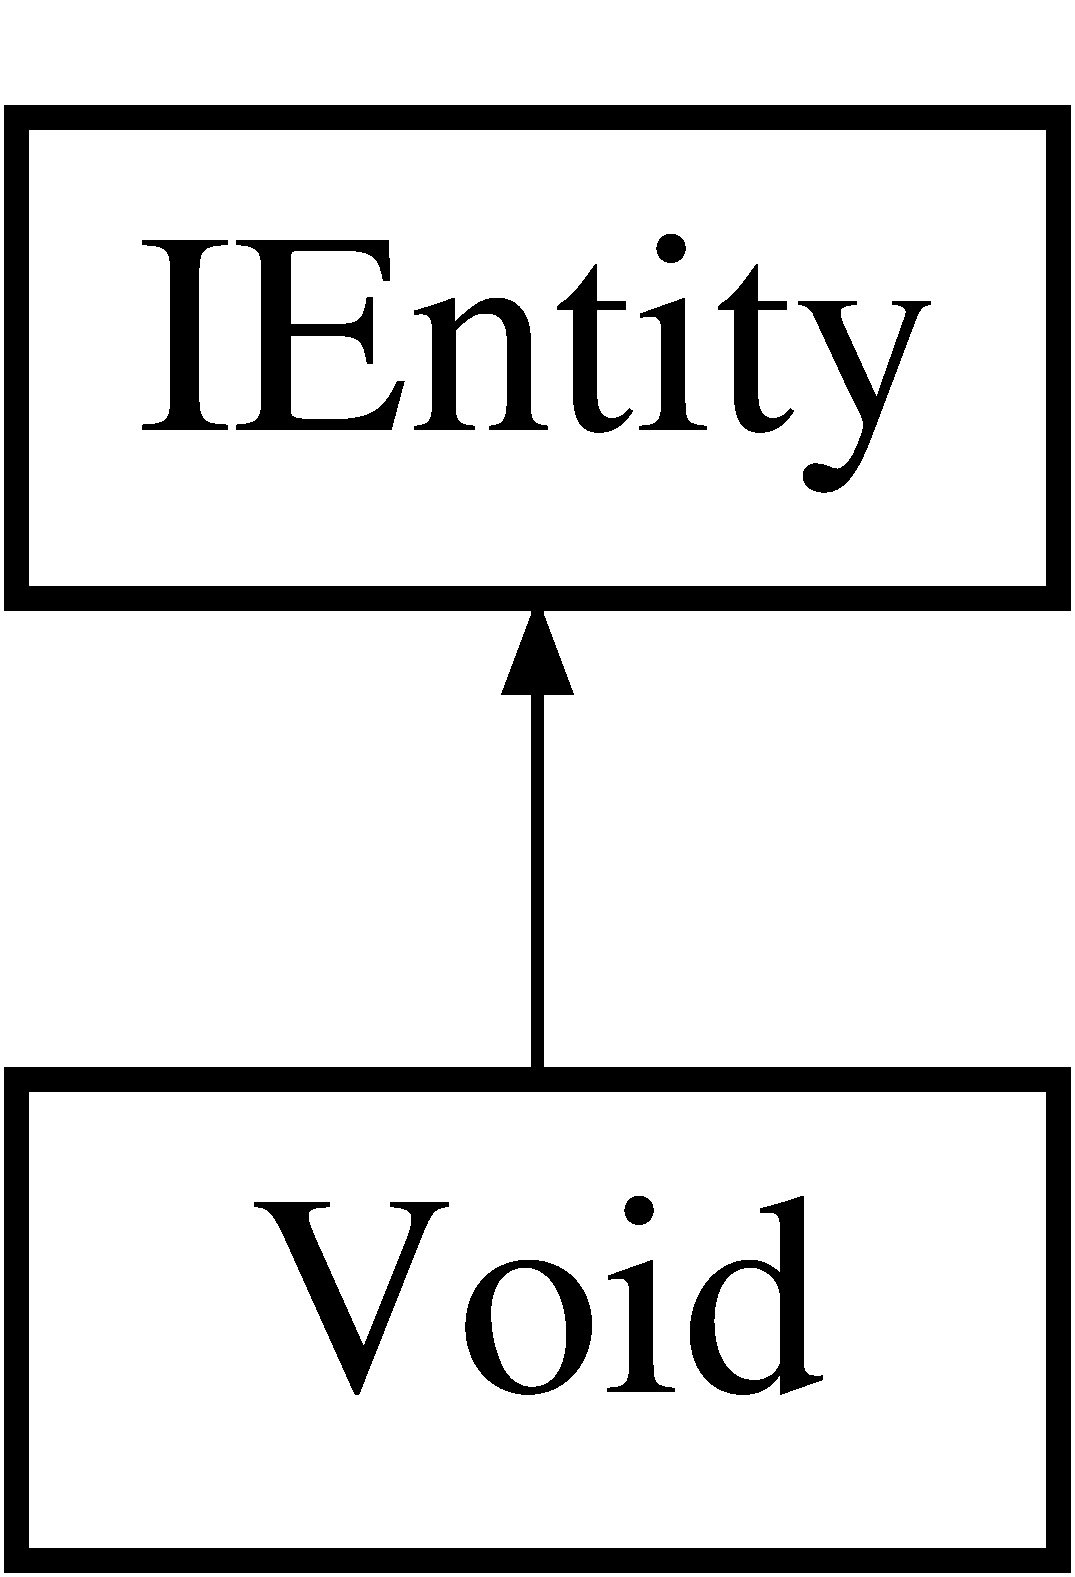
\includegraphics[height=2.000000cm]{class_void}
\end{center}
\end{figure}
\subsection*{Public Member Functions}
\begin{DoxyCompactItemize}
\item 
\mbox{\Hypertarget{class_void_ad3f67e2872db1519c236fdebd70a93f1}\label{class_void_ad3f67e2872db1519c236fdebd70a93f1}} 
std\+::string {\bfseries get\+Name} () final
\item 
\mbox{\Hypertarget{class_void_a6bb6ca3e97942ea5d04a15e794ae3e4b}\label{class_void_a6bb6ca3e97942ea5d04a15e794ae3e4b}} 
std\+::string {\bfseries get\+Color} () final
\end{DoxyCompactItemize}


The documentation for this class was generated from the following files\+:\begin{DoxyCompactItemize}
\item 
games/\+Snake/Void.\+hpp\item 
games/\+Snake/Void.\+cpp\end{DoxyCompactItemize}

\hypertarget{class_wall}{}\section{Wall Class Reference}
\label{class_wall}\index{Wall@{Wall}}
Inheritance diagram for Wall\+:\begin{figure}[H]
\begin{center}
\leavevmode
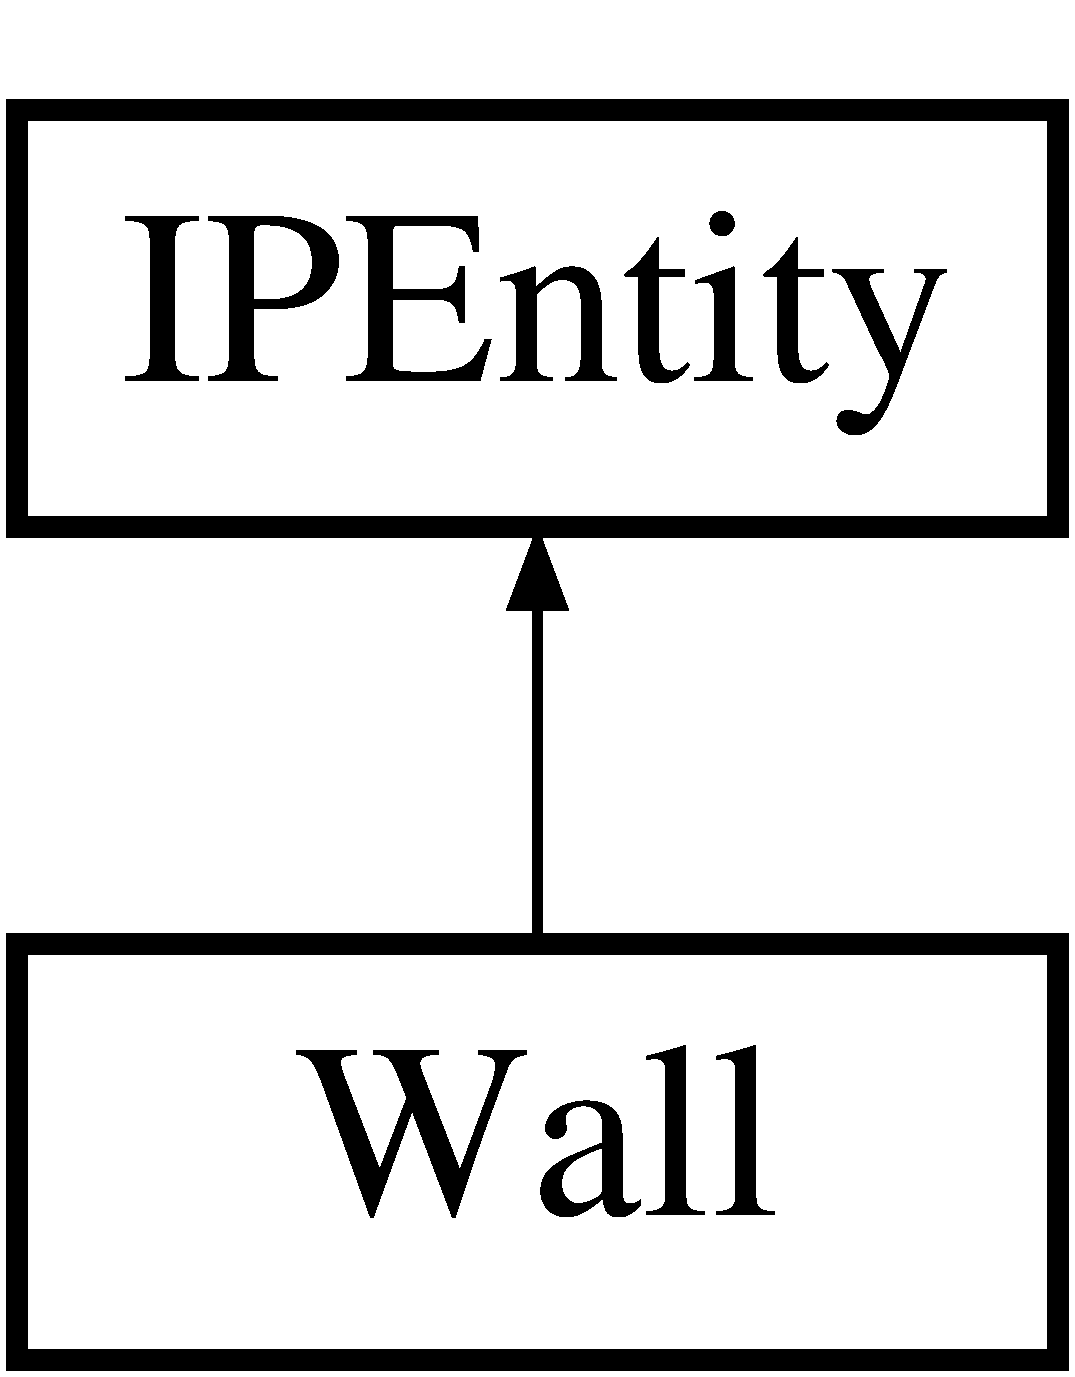
\includegraphics[height=2.000000cm]{class_wall}
\end{center}
\end{figure}
\subsection*{Public Member Functions}
\begin{DoxyCompactItemize}
\item 
\mbox{\Hypertarget{class_wall_a01988386e2cdb4edafcbb639de767aa4}\label{class_wall_a01988386e2cdb4edafcbb639de767aa4}} 
{\bfseries Wall} (\hyperlink{struct_vector2}{Vector2}$<$ int $>$ pos)
\item 
\mbox{\Hypertarget{class_wall_a8a5757082a516550531c6876acfb5b3f}\label{class_wall_a8a5757082a516550531c6876acfb5b3f}} 
\hyperlink{struct_vector2}{Vector2}$<$ int $>$ {\bfseries get\+Position} ()
\item 
\mbox{\Hypertarget{class_wall_a7d21f02285e92accf82f558120790013}\label{class_wall_a7d21f02285e92accf82f558120790013}} 
std\+::string {\bfseries get\+Name} ()
\item 
\mbox{\Hypertarget{class_wall_ac231beb8afadc9f83236a977162c73f8}\label{class_wall_ac231beb8afadc9f83236a977162c73f8}} 
std\+::string {\bfseries get\+Color} ()
\end{DoxyCompactItemize}


The documentation for this class was generated from the following files\+:\begin{DoxyCompactItemize}
\item 
games/\+Pac\+Man/Wall.\+hpp\item 
games/\+Pac\+Man/Wall.\+cpp\end{DoxyCompactItemize}

%--- End generated contents ---

% Index
\backmatter
\newpage
\phantomsection
\clearemptydoublepage
\addcontentsline{toc}{chapter}{Index}
\printindex

\end{document}
